%%%%%%%%%%%%%%%%%%%%%%%%%%%%%%%%%%%%%%%%%%%%%%%%%%%%%%%%%%%%%%%%%%%%%%%%%%%%%%%%
%%%%%%%%%%%%%%%%%%%%%%%%%%%%%%%%%%%%%%%%%%%%%%%%%%%%%%%%%%%%%%%%%%%%%%%%%%%%%%%%
%%                                                                            %%
%% thesistemplate.tex version 4.00 (2023/02/09)                               %%
%% The LaTeX template file to be used with the aaltothesis.sty (version 4.00) %%
%% style file.                                                                %%
%% This package requires pdfx.sty v. 1.5.84 (2017/05/18) or newer.            %%
%%                                                                            %%
%% This is licensed under the terms of the MIT license below.                 %%
%%                                                                            %%
%% Written by Luis R.J. Costa.                                                %%
%% Currently developed at Teacher services, Learning Services of Aalto        %%
%% University by Luis R.J. Costa since May 2019.                              %%
%%                                                                            %%
%% Copyright 2017-2021 aaltothesis.cls by Luis R.J. Costa,                    %%
%% luis.costa@aalto.fi.                                                       %%
%% Copyright 2017-2018 Swedish translations in aaltothesis.cls by Elisabeth   %%
%% Nyberg and Henrik Wallén henrik.wallen@aalto.fi.                           %%
%% Finnish documentation in the template opinnatepohja.tex translated from    %%
%% the English template documentation.                                        %%
%% Copyright 2021 English template thesistemplate.tex by Luis R.J. Costa,     %%
%% Maurice Forget, Henrik Wallén.                                             %%
%% Copyright 2018-2022 Swedish template kandidatarbetsbotten.tex by Henrik    %%
%% Wallen.                                                                    %%
%%                                                                            %%
%% Permission is hereby granted, free of charge, to any person obtaining a    %%
%% copy of this software and associated documentation files (the "Software"), %%
%% to deal in the Software without restriction, including without limitation  %%
%% the rights to use, copy, modify, merge, publish, distribute, sublicense,   %%
%% and/or sell copies of the Software, and to permit persons to whom the      %%
%% Software is furnished to do so, subject to the following conditions:       %%
%% The above copyright notice and this permission notice shall be included in %%
%% all copies or substantial portions of the Software.                        %%
%% THE SOFTWARE IS PROVIDED "AS IS", WITHOUT WARRANTY OF ANY KIND, EXPRESS OR %%
%% IMPLIED, INCLUDING BUT NOT LIMITED TO THE WARRANTIES OF MERCHANTABILITY,   %%
%% FITNESS FOR A PARTICULAR PURPOSE AND NONINFRINGEMENT. IN NO EVENT SHALL    %%
%% THE AUTHORS OR COPYRIGHT HOLDERS BE LIABLE FOR ANY CLAIM, DAMAGES OR OTHER %%
%% LIABILITY, WHETHER IN AN ACTION OF CONTRACT, TORT OR OTHERWISE, ARISING    %%
%% FROM, OUT OF OR IN CONNECTION WITH THE SOFTWARE OR THE USE OR OTHER        %%
%% DEALINGS IN THE SOFTWARE.                                                  %%
%%                                                                            %%
%%                                                                            %%
%%%%%%%%%%%%%%%%%%%%%%%%%%%%%%%%%%%%%%%%%%%%%%%%%%%%%%%%%%%%%%%%%%%%%%%%%%%%%%%%
%%                                                                            %%
%%                                                                            %%
%% An example for writting your thesis using LaTeX                            %%
%% Original version and development work by Luis Costa, changes to the text   %%
%% in the Finnish template by Perttu Puska.                                   %%
%% Support for Swedish added 15092014                                         %%
%% PDF/A-b support added on 15092017                                          %%
%% PDF/A-2 support added on 24042018                                          %%
%% Layout design and typesettin changed 15072021                              %%
%%                                                                            %%
%% This example consists of the files                                         %%
%%       thesistemplate.tex (version 4.00) (for text in English)              %%
%%       opinnaytepohja.tex (version 4.00) (for text in Finnish)              %%
%%       kandidatarbetsbotten.tex (version 1.10) (for text in Swedish)        %%
%%       aaltothesis.cls                                                      %%
%%       linediagram.pdf (graphics file)                                      %%
%%       curves.pdf      (graphics file)                                      %%
%%       ledspole.jpg    (graphics file)                                      %%
%%                                                                            %%
%%                                                                            %%
%% Typeset in Linux with                                                      %%
%% pdflatex: (recommended method)                                             %%
%%             $ pdflatex thesistemplate                                      %%
%%             $ pdflatex thesistemplate                                      %%
%%                                                                            %%
%%   The result is the file thesistemplate.pdf that is PDF/A compliant, if    %%
%%   you have chosen the proper \documenclass options (see comments below)    %%
%%   and your included graphics files have no problems.                       %%
%%                                                                            %%
%%                                                                            %%
%% Explanatory comments in this example begin with the characters %%, and     %%
%% changes that the user can make with the character %                        %%
%%                                                                            %%
%%%%%%%%%%%%%%%%%%%%%%%%%%%%%%%%%%%%%%%%%%%%%%%%%%%%%%%%%%%%%%%%%%%%%%%%%%%%%%%%
%%%%%%%%%%%%%%%%%%%%%%%%%%%%%%%%%%%%%%%%%%%%%%%%%%%%%%%%%%%%%%%%%%%%%%%%%%%%%%%%
%%
%% WHAT is PDF/A
%%
%% PDF/A is the ISO-standardized version of the pdf. The standard's goal is to
%% ensure that he file is reproducable even after a long time. PDF/A differs
%% from pdf in that it allows only those pdf features that support long-term
%% archiving of a file. For example, PDF/A requires that all used fonts are
%% embedded in the file, whereas a normal pdf can contain only a link to the
%% fonts in the system of the reader of the file. PDF/A also requires, among
%% other things, data on colour definition and the encryption used.
%% Currently three PDF/A standards exist:
%% PDF/A-1: based on PDF 1.4, standard ISO19005-1, published in 2005.
%%          Includes all the requirements essential for long-term archiving.
%% PDF/A-2: based on PDF 1.7, standard ISO19005-2, published in 2011.
%%          In addition to the above, it supports embedding of OpenType fonts,
%%          transparency in the colour definition and digital signatures.
%% PDF/A-3: based on PDF 1.7, standard ISO19005-3, published in 2012.
%%          Differs from the above only in that it allows embedding of files in
%%          any format (e.g., xml, csv, cad, spreadsheet or wordprocessing
%%          formats) into the pdf file.
%% PDF/A-4: based on PDF 2.0, standard ISO19005-4, published in November 2020.
%%
%% PDF/A-1 files are not necessarily PDF/A-2 -compatible and PDF/A-2 are not
%% necessarily PDF/A-1 -compatible.
%% Standards PDF/A-1, PDF/A-2 and PDF/A-3 have two levels:
%% b: (basic) requires that the visual appearance of the document is reliably
%%    reproduceable.
%% a (accessible) in addition to the b-level requirements, specifies how
%%   accessible the pdf file is to assistive software, say, for the physically
%%   impaired.
%% The PDF/A-4 standard does not have additional levels like in the earlier
%% standards.
%% For more details on PDF/A, see, e.g.,
%% https://www.loc.gov/preservation/digital/formats/fdd/fdd000318.shtml or
%% https://www.pdfa.org/resource/iso-19005-pdfa/
%%
%%
%% WHICH PDF/A standard should my thesis conform to?
%%
%% Either to the PDF/A-1b or the PDF/A-2b standard. If all the figures and
%% graphs used in thesis work do not require transparency features, use either
%% PDF/A-1b or PFDF/A-2b. If you have figures with transparency
%% characteristics, use the PDF/A-2b standard. However, drawing applications
%% often use the transparency parameter, setting it to zero, to specify opacity
%% and get the basic 2-D visualisation. As a result, validation of PDF/A-1b
%% will fail. Use PDF/A-2b if PDF/A-1b validation fails.
%% Do not use the PDF/A-3b standard for your thesis.
%% The font to be used are specified in this templatenand they should not be
%% changed. In addition to not adhering to Aalto's visual guidelines, you may
%% have difficulties in producing a PDF/A-compliant PDF.
%%
%%
%% Validate your PDF/A file at https://www.pdf-online.com/osa/validate.aspx
%%
%%
%% WHAT graphics format can I use to produce my PDF/A compliant file?
%%
%% When using pdflatex to compile your work, favour the use of pdf, but you can
%% use the jpg or png format especially for photographs. You will have PDF/A
%% compliance problems with figures in pdf if the fonts are not embedded in the
%% pdf file.
%% If you choose to use latex to compile your work, the only acceptable file
%% format for your figure is eps. DO NOT use the ps format for your figures.

%% USE one of the following three \documentclass set-ups:
%% * the first when using pdflatex to directly typeset your document in the
%%   chosen pdf/a format for online publishing (centred page layout),
%% * the second for one-sided printing your thesis with the layout (wide left
%%   margin), or
%% * the third for two-sided printing.
%%
\documentclass[english, 12pt, a4paper, sci, utf8, a-2b, online]{aaltothesis}
%\documentclass[english, 12pt, a4paper, sci, utf8, a-2b, print]{aaltothesis}
%\documentclass[english, 12pt, a4paper, sci, utf8, a-2b, print, twoside]{aaltothesis}

%% Use the following options in the \documentclass macro above:
%% your school: arts, biz, chem, elec, eng, sci
%% the character encoding scheme used by your editor: utf8, latin1
%% thesis language: english, finnish, swedish
%% make an archiveable PDF/A-1b or PDF/A-2b compliant file: a-1b, a-2b
%%                    (with pdflatex, a normal pdf containing metadata is
%%                     produced without the a-*b option)
%% typset for online document or print on paper: online, print
%%        online: typeset in symmetric layout and blue hypertext for online
%%                publishing
%%        print: typeset in a symmetric layout and black hypertext for printing
%%               on paper
%%          two-side printing: twoside (default is one-sided printing)
%%               typeset in a wide margin on the binding side of the page and
%%               black hypertext. Use with print only.
%%

%% Use one of these if you write in Finnish (or use the Finnish template
%% opinnaytepohja.tex)
%\documentclass[finnish, 12pt, a4paper, elec, utf8, a-1b, online]{aaltothesis}
%\documentclass[finnish, 12pt, a4paper, elec, utf8, a-1b, print]{aaltothesis}
%\documentclass[finnish, 12pt, a4paper, elec, utf8, a-1b, print, twoside]{aaltothesis}

%% Use one of these if you write in Swedish (or use the Swedish template
%% kandidatarbetsbotten.tex)
%\documentclass[swedish, 12pt, a4paper, elec, utf8, a-2b, online]{aaltothesis}
%\documentclass[swedish, 12pt, a4paper, elec, utf8, a-2b]{aaltothesis}
%\documentclass[swedish, 12pt, a4paper, elec, dvips, online]{aaltothesis}

%% FOR USERS OF AMS PACKAGES:
%% * newtxmath used in this template loads amsmath, so
%%   you needn't load it. If you want to use options in amsmath, load it here,
%%   before \setupthesisfonts below to pass the options to amsmath.
%% * If you want to use amsthm, load it here before \setupthesisfonts to avoid
%%   a clash with newtxmath.
%% * If using amsmath with options and you want to use amsthm, load amsthms
%%   after amsmath, as described in the amsthm documentation.
%% * Don't use amsbsym or amsfonts. The symbols [and macros] there are defined in
%%   newtxmath and so clash if used.
%\usepackage[options]{amsmath}
%\usepackage{amsthm}

%% DO NOT MOVE OR REMOVE \setupthesisfonts
\setupthesisfonts

%% Add here the packges you need
\usepackage{graphicx}

% Tables
\usepackage{tabularx,ragged2e}
\newcolumntype{C}{>{\Centering\arraybackslash}X} % centered "X" column
\usepackage{enumitem}
\usepackage{float}

% Code snippets
% \usepackage[usenames,dvipsnames]{xcolor}
\usepackage{listings}
\usepackage{soul}

\definecolor{codegreen}{rgb}{0,0.5,0}
\definecolor{codepurple}{rgb}{0.69,0,0.86}
\definecolor{codered}{rgb}{0.64,0.08,0.08}
\definecolor{codeteal}{rgb}{0,0.44,0.76}
\definecolor{codeyellow}{rgb}{0.48,0.37,0.15}
\definecolor{codedarklime}{rgb}{0.04,0.53,0.35}

\definecolor{darkred}{rgb}{0.5,0,0}
\definecolor{bgcolor}{rgb}{0.95,0.95,0.92}

\newcommand\YAMLcolonstyle{\color{black}\mdseries}
\newcommand\YAMLkeystyle{\color{darkred}\mdseries}
\newcommand\YAMLvaluestyle{\color{blue}\mdseries}

\makeatletter

%% Feedback macros
\newcommand{\mycomment}[3]{\textcolor{#1}{#2:~#3}}
\newcommand{\jb}[1]{\noindent\mycomment{aaltoRed}{JB}{#1}}

% here is a macro expanding to the name of the language
% (handy if you decide to change it further down the road)
\newcommand\language@yaml{yaml}

\expandafter\expandafter\expandafter\lstdefinelanguage
\expandafter{\language@yaml}
{
  % assuming a key comes first
  basicstyle=\YAMLkeystyle,
  sensitive=false,
  comment=[l]{\#},
  morecomment=[s]{/*}{*/},
  commentstyle=\color{codegreen}\ttfamily,
  stringstyle=\YAMLvaluestyle\ttfamily,
  moredelim=[l][\color{orange}]{\&},
  moredelim=[l][\color{orange}]{*},
  % switch to value style at :
  moredelim=**[il][\YAMLcolonstyle{:}\YAMLvaluestyle]{:},
  literate =    {---}{{\ProcessThreeDashes}}3
                {>}{{\textcolor{codered}\textgreater}}1
                {|}{{\textcolor{codered}\textbar}}1
                {\ -\ }{{\mdseries\ -\ }}3,
}

% switch to key style at EOL
\lst@AddToHook{EveryLine}{\ifx\lst@language\language@yaml\YAMLkeystyle\fi}
\makeatother

\newcommand\ProcessThreeDashes{\llap{\color{black}\mdseries-{-}-}}

\lstdefinelanguage{javascript}{
  keywords={import, export, try, catch, return, throw, switch, case, if, while, do, else, break, await},
  ndkeywords={class, implements, typeof, function, this, new, true, false, null, boolean, const, var, in, async, =>},
  sensitive=false,
  comment=[l]{//},
  morecomment=[s]{/*}{*/},
  morestring=[b]',
  morestring=[b]",
  morestring=[b]`
}

\lstdefinelanguage{json}{
  basicstyle=\YAMLkeystyle, % assuming a key comes first
  sensitive=false,
  moredelim=[l][\color{orange}]{\&},
  moredelim=[l][\color{orange}]{*},
  moredelim=**[il][\YAMLcolonstyle{:}\YAMLvaluestyle]{:}, % switch to value style at :
  morestring=[b]',
  morestring=[b]",
  literate =    {---}{{\ProcessThreeDashes}}3
                {>}{{\textcolor{codered}\textgreater}}1
                {|}{{\textcolor{codered}\textbar}}1
                {\ -\ }{{\mdseries\ -\ }}3,
}

\lstdefinelanguage{Docker}{
  keywords={FROM, USER, ADD, RUN, COPY, WORKDIR, ENTRYPOINT, CMD},
  sensitive=false,
  comment=[l]{\#},
  morestring=[b]',
  morestring=[b]"
}

\lstdefinelanguage{bash}{
  keywords={if, while, do, else, done},
  ndkeywords={set, echo, cut, nsenter, docker, iptables},
  sensitive=false,
  comment=[l]{\#},
  morestring=[b]',
  morestring=[b]"
}

\lstdefinestyle{mystyle}{
    backgroundcolor=\color{bgcolor},
    commentstyle=\color{codegreen},
    keywordstyle=\color{codepurple},
    ndkeywordstyle=\color{blue},
    numberstyle=\tiny\color{gray},
    stringstyle=\color{codered},
    basicstyle=\footnotesize,
    breakatwhitespace=false,
    breaklines=true,
    captionpos=b,
    keepspaces=true,
    numbers=left,
    numbersep=5pt,
    showspaces=false,
    showstringspaces=false,
    showtabs=false,
    tabsize=2
}

\lstset{style=mystyle}

% \usepackage{amsfonts,amssymb,amsbsy,csquotes}
\usepackage{csquotes}
\usepackage{biblatex}
\addbibresource{./refs.bib}

% \usepackage{hyperref}
% \hypersetup{pdfpagemode=UseNone, pdfstartview=FitH,
%   colorlinks=true,urlcolor=red,linkcolor=blue,citecolor=black,
%   pdftitle={Default Title, Modify},pdfauthor={Your Name},
%   pdfkeywords={Modify keywords}}

%% For tables that span multiple pages; used to split a paraphrasing example in the appendix. If you don't need it, remove it.
\usepackage{longtable}

%% A package for generating Creative Commons copyright terms. If you don't use the CC copyright terms, remove it, since otherwise undesired information may be added to this document's metadata.
\usepackage[type={CC}, modifier={by-nc-sa}, version={4.0}]{doclicense}
%% Find below three examples for typesetting the CC license notice.

%% Edit to conform to your degree programme
%% Capitalise the words in the name of the degree programme: it's a name
\degreeprogram{Computer, Communication and Information Sciences}

%% Your major
\major{Computer Science}

%% Choose one of the three below
%\univdegree{BSc}
\univdegree{MSc}
%\univdegree{Lic}

\thesisauthor{Aarni Halinen}

%% Your thesis title and possible subtitle comes here and possibly, again, together with the Finnish or Swedish abstract. Do not hyphenate the title (and subtitle), and avoid writing too long a title. Should LaTeX typeset a long title (and/or subtitle) unsatisfactorily, you might have to force a linebreak using the \\ control characters. In this case...
%% * Remember, the title should not be hyphenated!
%% * A possible 'and' in the title should not be the last word in the line; it begins the next line.
%% * Specify the title (and/or subtitle) again without the linebreak characters in the optional argument in box brackets. This is done because the title is part of the metadata in the pdf/a file, and the metadata cannot contain linebreaks.
\thesistitle{Kubernetes inter-pod container isolation}
% \thesistitle[Title of the thesis]{Title of\\ the thesis}
%% Either remove or leave \thesissubtitle{} empty if you don't use it \thesissubtitle{A possible subtitle}
% \thesissubtitle{}

\place{Espoo}

%% The date for the bachelor's thesis is the day it is presented
\date{1 June 2023}

%% Thesis supervisor
%% Note the "\" character in the title after the period and before the space and the following character string. This is because the period is not the end of a sentence after which a slightly longer space follows, but what is desired is a regular interword space.
\supervisor{Prof.\ Mario Di Francesco}

%% Advisor(s)---two at the most---of the thesis. Check with your supervisor how many official advisors you can have.
\advisor{M.Sc.\ (Tech.)\ José\ Luis\ Martin\ Navarro}
\advisor{M.Sc.\ (Tech.)\ Jacopo\ Bufalino}

%% If you do your thesis work in a company of other institute, give the name of the company or instution here. Otherwise, leave the macro empty, comment it out, or remove it. This will remove this field from the abstract page.
% \collaborativepartner{Company or institute name}

%% Aaltologo: syntax:
%% \uselogo{?|!|''}
%% The logo language is set to be the same as the thesis language.
%\uselogo{?}
%\uselogo{!}
\uselogo{''}

%%%%%%%%%%%%%%%%%%               COPYRIGHT TEXT               %%%%%%%%%%%%%%%%%%
%%%%%%%%%%%%%%%%%%%%%%%%%%%%%%%%%%%%%%%%%%%%%%%%%%%%%%%%%%%%%%%%%%%%%%%%%%%%%%%%

%% Copyright of a work is with the creator/author of the work regardless of
%% whether the copyright mark is explicitly in the work or not. You may, if you
%% wish---we encourage you to do so---publish your work under a Creative
%% Commons license (see creativecommons.org), in which case the license text
%% must be visible in the work. Write here the copyright text you want using the
%% macro \copyrighttext, which writes the text into the metadata of the pdf file
%% as well.
%%
%% Syntax:
%% \copyrigthtext{metadata text}{text visible on the page}
%%
%% CHOOSE ONE OF THE COPYRIGHT NOTICE STYLES BELOW.
%% IF USING THE CC TERMS, CHOOSE THE LICENSE YOU WANT TO USE.
%% The different CC licenses are listed at
%% https://creativecommons.org/about/cclicenses/.
%% If you use the icons from the dolicense.sty package, add the package above
%% (\usepackage{dolicense}).
%% IMPORTANT NOTE!! Manually write the CC text in the \copyrighttext metadata
%% text field.
%%
%% NOTE: In the macros below, the text written in the metadata must have a
%% \noexpand macro before the \copyright special character. When not in pdf/a
%% mode (i.e. a-1b or a-2b are not specified in \documentclass), two \noexpands
%% are required in the metadata text to correctly render the copyright mark in
%% the pdf metadata. In pdf/a mode one \noexpand suffices.
%%
%% EXAMPLE OF PLAIN COPYRIGHT TEXT
%% The macros \copyright and \year below must be separated by the \ character
%% (space chacter) from the text that follows. The macros in the argument of the
%% \copyrighttext macro automatically insert the year and the author's name.
%% (Note! \ThesisAuthor is an internal macro of the aaltothesis.cls class file).
%%
%\copyrighttext{Copyright \noexpand\textcopyright\ \number\year\ \ThesisAuthor}
%{Copyright \textcopyright{} \number\year{} \ThesisAuthor}
%%
%% Of course, the same text could have simply been written as
%% \copyrighttext{Copyright \noexpand\copyright\ 2018 Eddie Engineer}
%% {Copyright \copyright{} 2022 Eddie Engineer}
%%
%% EXAMPLES OF CC LICENSE: different ways to display the same license
%% 1. A simple Creative Commons license text with a link to the copyright notice:
%\copyrighttext{\noexpand\textcopyright\ \number\year. This work is
%	licensed under a CC BY-NC-SA 4.0 license.}{\textcopyright{}
%	\number\year. This work is licensed under a
%	\href{https://creativecommons.org/licenses/by-nc-nd/4.0/}{CC BY-NC-SA 4.0}
%	license.}
%
%% To get the URL of the license of your choice, go to
%% https://creativecommons.org/about/cclicenses/, click on the chosen license
%% you want to use, and copy-and-paste the URL in the macro \href above.
%%
%% 2. A short Creative Commons license text containing the respective CC icons
%% (requires the package dolicense.sty to be added in the preamble as done
%% above) and a link to the corresponding Creative Commons license webpage (see
%% the dolicense package documentation for other license icons):
%\copyrighttext{\noexpand\textcopyright\ \number\year. This work is licensed
%	under a CC BY-NC-SA 4.0 license.}{
%	\parbox{95mm}{\noindent\textcopyright\ \number\year. \doclicenseText}
%	\hspace{1em}\parbox{35mm}{\doclicenseImage}
%}
%%
%% 3. An expanded Creative Commons license text containing the respective CC
%% icons text and as generated by the dolicense.sty package (the license is set
%% via package options in \usepackage[options]{dolicense} above; see the
%% dolicense package documentation for other license texts and icons):
\copyrighttext{\noexpand\textcopyright\ \number\year. This work is licensed under a Creative Commons "Attribution-NonCommercial-ShareAlike 4.0 International" (BY-NC-SA 4.0) license.}{\noindent\textcopyright\ \number \year \ \doclicenseThis}
%%%%%%%%%%%%%%%%%%%%%%%%%%%%%%%%%%%%%%%%%%%%%%%%%%%%%%%%%%%%%%%%%%%%%%%%%%%%%%%%


%% The English abstract:
%% All the details (name, title, etc.) on the abstract page appear as specified
%% above.
%% Thesis keywords:
%% Note! The keywords are separated using the \spc macro
\keywords{Kubernetes, Container, Docker, Security}

%% The abstract text. This text is included in the metadata of the pdf file as well as the abstract page.
\thesisabstract{
The abstract is a short description of the essential contents of the thesis:
what was studied and how and what were the main findings. For a Finnish thesis,
the abstract should be written in both Finnish and English; for a Swedish
thesis, the abstract should be written in both Swedish and English. The abstracts for English theses written by
Finnish or Swedish speakers should be written in English and either in Finnish
or in Swedish, depending on the student’s language of basic education. Students
educated in languages other than Finnish or Swedish write the abstract only in
English. Students may include a second or third abstract in their native
language, if they wish.
The abstract text of this thesis is written on the readable abstract page and in the pdf file's metadata via the thesisabstract macro (see the
comment in the TeX file). Write in this the text that goes into the metadata. The
metadata cannot contain special characters, linebreak or paragraph break
characters, so these must not be used here. If your abstract does not contain
special characters and does not require paragraphs, you may take advantage of
the abstracttext macro (see the comment in the TeX file below). Otherwise, the
metadata abstract text must be identical to the text on the abstract page.
}

%% You can prevent LaTeX from writing into the xmpdata file (it contains all the metadata to be written into the pdf file) by setting the writexmpdata switch to 'false'. This allows you to write the metadata in the correct format directly into the file thesistemplate.xmpdata.
% \setboolean{writexmpdatafile}{false}

%% All that is printed on paper starts here
\begin{document}

%% Create the coverpage
\makecoverpage

%% Typeset the copyright text.
%% If you wish, you may leave out the copyright text from the human-readable page of the pdf file. This may seem like a attractive idea for the printed document especially if "Copyright (c) yyyy Eddie Engineer" is the only text on the page. However, the recommendation is to print this copyright text.
\makecopyrightpage

\clearpage
%% Note that when writing your thesis in English, place the English abstract first followed by the possible Finnish or Swedish abstract.

%% Abstract text
%% All the details (name, title, etc.) on the abstract page appear as specified above.

%% The text in the \thesisabstract macro is stored in the macro \abstractext, so you can use the text metadata abstract directly as follows:
\begin{abstractpage}[english]
  \abstracttext{}
\end{abstractpage}

%% Force a new page so that the possible Finnish or Swedish abstract does not begin on the same page
\newpage
%% Abstract in Finnish.  Delete if you don't need it.
%% Respecify those fields that differ from the earlier specification or simply respecify all fields.
\thesistitle{Opinnäyteen otsikko}
% \thesissubtitle{Opinnäytteen mahdollinen alaotsikko}
\supervisor{Prof.\ Mario Di Francesco}
\advisor{DI José\ Luis\ Martin\ Navarro}
\advisor{DI Jacopo\ Bufalino}
% \degreeprogram{Elektroniikka ja sähkötekniikka}
% \major{Sopiva pääaine}
% \collaborativepartner{Yhtiön tai laitoksen nimi}
\date{1.6.2023}
%% The keywords need not be separated by \spc now.
\keywords{Vastus, resistanssi, lämpötila}
%% Abstract text
\begin{abstractpage}[finnish]
Tiivistelmä on lyhyt kuvaus työn keskeisestä sisällöstä: mitä tutkittiin ja
miten sekä mitkä olivat tärkeimmät tulokset. Suomenkielisen opinnäytteen
tiivistelmä kirjoitetaan suomeksi ja englanniksi ja ruotsinkielisen vastaavasti
ruotsiksi ja englanniksi. Suomen- tai ruotsinkielisten opiskelijoiden, joiden
opinnäytteen kieli on englanti, tulee kirjoittaa tiivistelmänsä englanniksi ja
koulusivistyskielellään. Muiden kuin koulusivistyskieleltään suomen- tai
ruotsinkielisten tulee kirjoittaa tiivistelmänsä vain englanniksi. Opiskelija
voi halutessaan lisätä opinnäytteeseensä toisen tai kolmannen tiivistelmän
omalla äidinkielellään.
Tämän opinnäytteen tiivistelmäteksti kirjoitetaan opinnäytteen luettavan osan
lomakkeen lisäksi myös pdf-tiedoston metadataan. Kirjoita tähän metadataan
kirjoitettavaa teksti. Metadatatekstissa ei saa olla erikoismerkkejä,
rivinvaiho- tai kappaleenjakomerkkiä, joten näitä merkkeja ei saa käyttää tässä.
Jos tiivistelmäsi ei sisällä erikoimerkkejä eikä kaipaa kappaleenjakoa, voit
hyödynttää makroa abstracttext luodessasi lomakkeen tiivistelmää (katso
kommentti tässä TeX-tiedostossa alla). Metadatatiivistelmatekstin on muuten
oltava sama kuin lomakkeessa oleva teksti.

\end{abstractpage}

%% Force new page so that the Swedish abstract starts from a new page
\newpage

\dothesispagenumbering{}

%% Preface
%% This section is optional. Remove it if you do not want a preface.
\mysection{Preface}
% \mysection{Esipuhe}
I want to thank Professor Pirjo Professor and my instructors Dr Alan Advisor and
Ms Elsa Expert for their guidance.

I also want to thank my partner for keeping me sane and alive.

\vspace{5cm}
Otaniemi, 9 February 2023 \\

\vspace{5mm}
{\hfill Aarni O.\ Halinen \hspace{1cm}}

%% Force a new page after the preface
\newpage

%% Table of contents.
\thesistableofcontents

\mysection{Abbreviations}

\begin{tabular}{ll}
  API         & Application Programming Interface   \\
  BGP         & Border Gateway Protocol             \\
  BPF, cBPF   & (classic) Berkeley Packet Filter    \\
  cgroups     & Control groups                      \\
  CLI         & Command-line interface              \\
  CNCF        & Cloud Native Computing Foundation   \\
  CNI         & Container Network Interface         \\
  CRD         & Custom Resource Definition          \\
  DAC         & Discretionary Access Control        \\
  DoS         & Denial of Service                   \\
  eBPF        & Extended Berkeley Packet Filter     \\
  gRPC        & Google Remote Procedure Call        \\
  HTTP        & Hypertext Transfer Protocol         \\
  IPAM        & IP Address Management               \\
  IPC         & Inter-process communication         \\
  K8s         & Kubernetes                          \\
  LXC         & Linux Containers                    \\
  MAC         & Mandatory Access Control            \\
  NAT         & Network Address Translation         \\
  NIC         & Network Interface Controller        \\
  OOM         & Out-of-memory                       \\
  OpenVZ      & Open Virtuozzo                      \\
  OS          & Operating System                    \\
  PID         & Process ID                          \\
  RCE         & Remote code execution               \\
  SELinux     & Security-Enhanced Linux             \\
  Seccomp     & Secure computing mode               \\
  TC          & Traffic Control                     \\
  VXLAN       & Virtual Extensible LAN              \\
  XDP         & eXpress Data Path                   \\
  ZTA         & Zero Trust Architecture             \\
\end{tabular}


%% \clearpage is similar to \newpage, but it also flushes the floats (figures and tables).
\cleardoublepage

%% Leave page number of the first page empty
\thispagestyle{empty}

%% Text body begins.
\section{Introduction} \label{sec:intro}

During the last decade, the IT industry has shifted from monolithic software applications towards microservices. In the microservice architecture, each application is split into a suite of smaller independent services that handle part of the business logic \cite{fowler2014microservices}. Each service runs its own process, and the application data is sent between the components using lightweight communication mechanisms such as Hypertext Transfer Protocol (HTTP) and Google Remote Procedure Call (gRPC).
This architectural approach also increases software agility because each service becomes an independent unit of development, deployment, operations, versioning, and scaling \cite{jamshidi2018microservices}. This modularity is often associated with benefits like faster delivery and improved scalability.
\jb{The point is that microservices have become popular because of containers}
During the same period of time, containers have become a widely used method to deploy applications. Containers are a lightweight virtualization technique in which the application is bundled with all its dependencies into a single deployable unit that executes on top of the host machine kernel \cite{bui2015analysis}. As such, a single microservice is quite often built and deployed as a container. In more complex systems with multiple containers, an orchestrator is often used to manage workloads. Kubernetes is one of the most widely used orchestrator tools.
\jb{Describe shortly what an orchestrator does and what is the difference between orchestrator and container runtime. Maybe this should be in the background.}

Similarly to how design patterns emerged from the birth of object-oriented software systems, the modularity of containers and microservices has allowed the development of distributed system design patterns \cite{burns2016design}.
The most common of these patterns is the sidecar pattern, in which peripheral tasks like logging and observability are split away as their own containers from the main application container.
The pattern allows easier installation of these nonfunctional features, while also keeping them away from the main container's source code.
Basically, the sidecar pattern is an extension of the modularity of the microservices architecture inside the microservice itself.
The benefits of sidecar pattern are similar to microservices, allowing better resource allocation, re-use of components in other services and provide a failure containment boundary, for example.
In Kubernetes, the basic unit of deployment is called a Pod, which may include one or more co-scheduled containers.
The Pod is analogous to a microservice, while it contains one main container and all its sidecars bundled into one deployable unit.

\subsection{Problem Statement}

Although the sidecar pattern makes it easier to add peripheral tasks to applications, it opens up questions about application security. Quite often, developers rely on containers created by third parties for sidecar tasks. The source code of these sidecar containers is not always available and finding vulnerabilities therein is not a trivial task. Furthermore, malicious actors can use supply chain attacks and typo-squatting to trick victims into installing malicious sidecars to their clusters. Once malicious attackers gain access to the sidecar, any misconfigurations or permissive security mechanisms put the whole cluster at risk. Furthermore, Kubernetes is not secure by default; on a fresh installation, most of the included security mechanisms are in permissive settings or outright disabled.

In Kubernetes, there is limited amount of security features available on container-level. Most of the security-related policies and capabilities are defined for the Pod, which essentially means that any capability required by the main application is inherited in the sidecar. Thus, any privileged workload, even in another container in the Pod, risks privilege escalation from the sidecar. In addition, Kubernetes' firewalling solution, Network Policies, are granted for the whole Pod instead of individual containers. Both of the aforementioned issues allow for lateral movement and further escalation for the attackers. Thus, any exploitable security issue in a sidecar container makes an optimal launchpad for attack against the whole cluster.
\jb{Statements are too weak. Here, the reader should understand that sidecars may contain vulnerable (or potentially vulnerable) code, and there are NO mechanisms to protect containers running in the same Pod.}

Zero trust architecture and the principle of least privilege are common security paradigms for limiting lateral movement and further escalation in a system if any component within has been compromised. In both paradigms, the capabilities of an individual component are limited to only those that are required for the component to function. The capabilities, such as network access and any container privileges, are explicitly given to the component that requires them, while everything else is denied.

If these paradigms are successfully applied to sidecars, sidecars could only use operations and network access required, while anything else would be blocked. However, since Kubernetes provides limited security on container-level, we need to find some other ways to implement these paradigms inside the Pods. This thesis proposes a solution for restricting the capabilities of sidecar while minimally affecting the main container, thus improving the security by extending the paradigms within the Pod.

\subsection{Thesis outline}

The following Chapter~\ref{sec:bg} gives background about containers, Kubernetes and explains their common attack vectors. It also discusses Kubernetes networking and container network interface plugins. Chapter~\ref{sec:methods} proposes ideas for isolating sidecars from the main application container. The chapter discusses both container and network security in the context of Kubernetes Pod. Chapter~\ref{sec:solution} introduces an implementation based on the findings of the previous chapter. The pros and cons of the solution are discussed in Chapter~\ref{sec:discussion}. Finally, Chapter~\ref{sec:conclusion} discusses future research and concludes the thesis.

\clearpage

\section{Background} \label{sec:bg}

\subsection{Zero trust architecture}

% Conventional network security has focused on perimeter defense. Historically, most corporate resources have been located within and protected by the enterprise’s network perimeter, which tended to be large and static. Subjects that are inside the network perimeter are often assumed to be implicitly trusted and are given broad access to the corporate resources within the network perimeter. Attempts to access resources from outside the network perimeter, i.e., from the internet, are often subject to more scrutiny than those originating from within. However, a subject can be compromised regardless of whether it is inside or outside of the network perimeter. Once a subject is compromised, malicious actors—through impersonation and escalation—can gain access to the resources that the subject is authorized to access and move laterally within the network perimeter to access adjacent corporate resources.

Conventional network security has historically focused on perimeter defense \cite{kerman2020implementing}.
Subjects like workload resources and users inside the perimeter are often assumed to be trusted and implicitly given access inside the network, while any request originating outside the network is subject to more scrutiny.
Although the systems seem initially secure, the modern IT landscape with cloud-based systems, third-party components, remote workers, etc. increases the attack surface of threat actors.
Once any subject inside the perimeter is compromised, the attackers can gain access to all the resources that the subject is authorized to access and move laterally within the perimeter, escalating the attack on other resources.

%By protecting each resource individually and employing extensive identity, authentication, and authorization measures to verify a subject’s requirement to access each resource, zero trust can ensure that authorized users, applications, and systems have access to only those resources that they absolutely have a need to access in order to perform their duties, not to a broad set of resources that all happen to be within the network perimeter. This way, if a malicious actor does manage to gain unauthorized access to one resource, this access will not provide them with any advantage when trying to move laterally to other nearby resources. To compromise those other resources, the attacker would be required to figure out how to circumvent the mechanisms that are protecting those resources individually because it is not possible to reach those resources from nearby compromised resources. In this way, ZTA limits the insider threat because instead of having permission to access all resources within the network perimeter, malicious insiders would only be permitted to access those resources they require to perform their official roles.

Zero trust architecture (ZTA) is a security paradigm that focuses on data and resource protection and on the premise that trust must always be explicitly granted and continuously evaluated \cite{kerman2020implementing, rose2020zero}. In contrast to a single perimeter defense, the focus in ZTA is to create fine-grained access rules around each of the resources while at the same time enforcing rules that deny other access, which is not explicitly allowed. Following the principle of least privilege, the access rules are made as granular as possible so that the number of trusted subjects equals the actual number of subjects that require the access. This achieves a multi-layered security boundaries, where the breach of one component through the most outward perimeter does not compromise the whole system. Instead of having permission to access all resources within the perimeter, malicious actors could only laterally move to the resources that the compromised component required to function. Any other component is still protected by its own perimeter, which would require another successful attack to be breached. Thus, the compromised component is of limited usefulness to the attacker instead of serving as a general attack vector against the system.
\jb{How is the Zero trust implemented in practice? Is there a relationship between zero trust and sidecars?}

\subsection{Containerization and Docker}

\begin{figure}[h!]
  \centering
  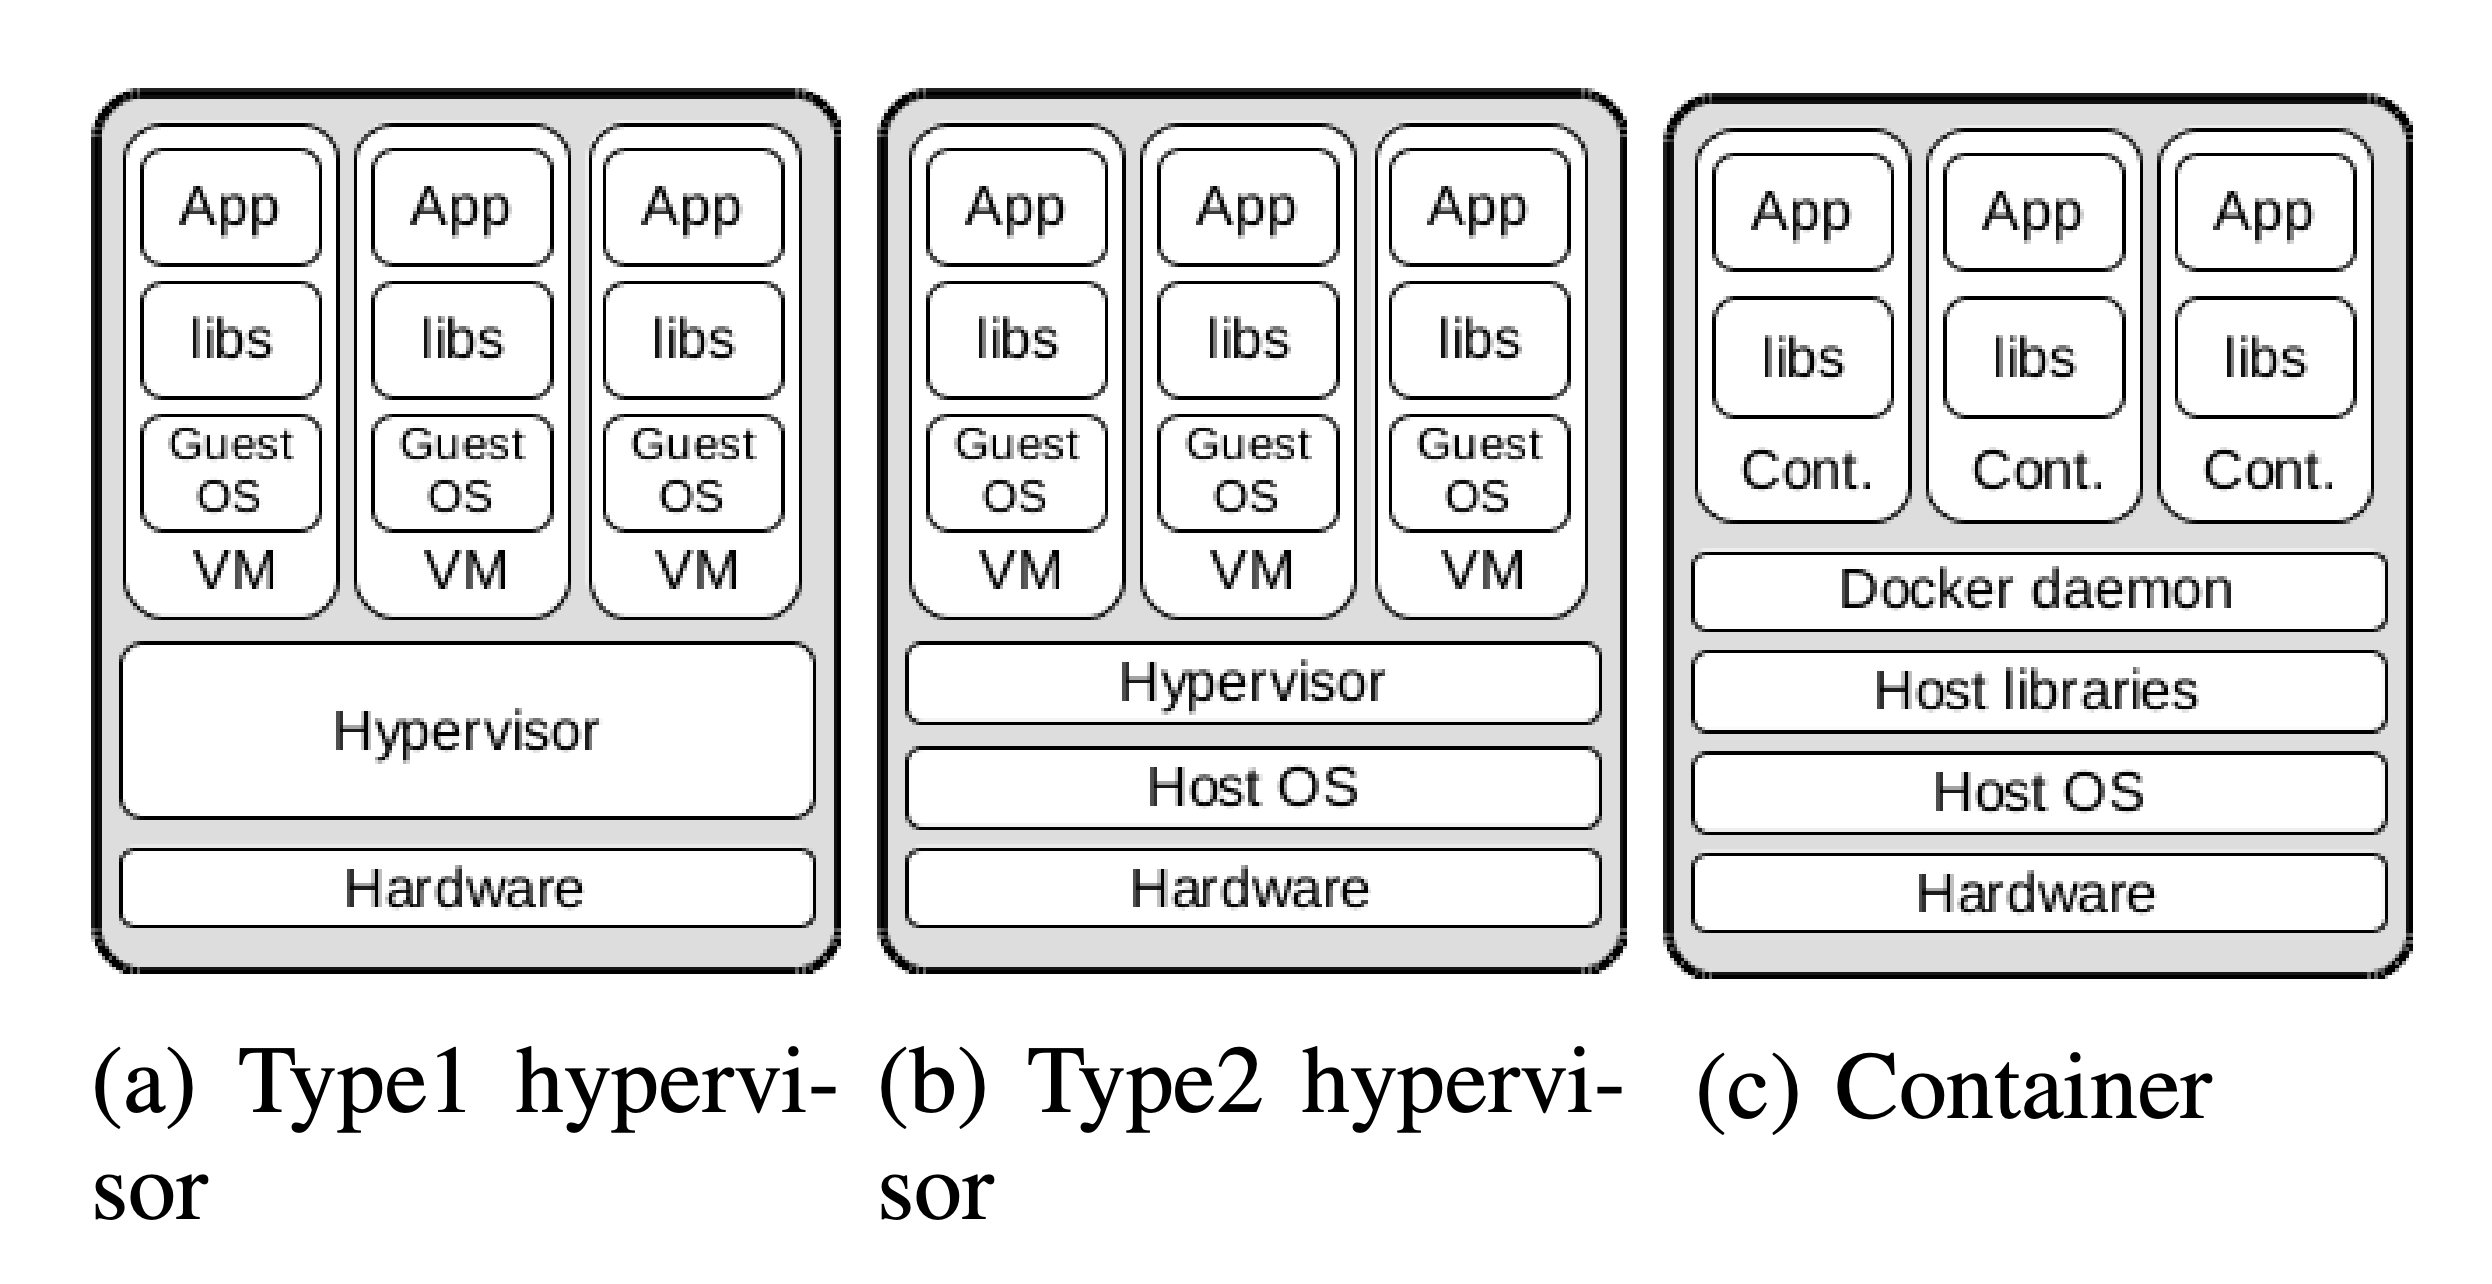
\includegraphics[width=\linewidth]{files/figure-1.png}
  \caption{Virtualization models \cite{combe2016docker}} % The image does not render nicely, would you be able to make one from scratch or find an SVG?
  \label{figure-1}
\end{figure}

Figure~\ref{figure-1} illustrates common virtualization models. While traditional virtualization techniques virtualize workloads on top of a hypervisor that shares hardware resources between virtual machines, containerization is a technique where virtualization occurs at the operating system level \cite{merkel2014docker}. Processes executing in containers run on the kernel of the host machine. However, each container is isolated to its own network, process namespace, and so on; two containers on the same host OS do not know that they share resources. Furthermore, containers are similarly isolated from accessing host OS resources.

BSD jails and \textit{chroot} can be considered early forms of containerization technology, so the idea of containers is not new \cite{combe2016docker}. Recent Linux container solutions rely on two main implementations: Linux Containers (LXC) -based solution that relies on kernel features such as control groups (cgroups) and namespaces, and a custom kernel and Linux distribution called Open Virtuozzo (OpenVZ). Docker \cite{docker} is a hugely popular LXC-based container runtime and provides an easy-to-use API and tooling for creating and managing containers. Docker also provides containerization for other OSes as well. However, in this thesis we focus only on the Linux implementation.

\subsubsection{Linux containers}

The Linux containers technology implements container isolation and containment using a Linux kernel feature called namespaces \cite{lin2018measurement}. Namespaces \cite{manpages-namespace} are a construct that wraps a global system resource in an abstraction that makes it appear to the processes in the namespace that they have their own isolated instance of the global resource. There are a total of eight namespaces: i) \textit{Cgroup} which is used for resource management, ii) \textit{Inter-process communication} (IPC) that isolates POSIX message queues, etc., iii) \textit{Network} which isolates network devices, stack ports, etc., iv) \textit{Mount} for file system isolation, v) \textit{Process ID} (PID), vi) \textit{Time}, vii) \textit{User} for isolating user and group identifiers, and viii) \textit{UTS} which isolates hostnames and NIS domain names. For example, the \textit{network} namespace provides each container with its own loopback device, and even \texttt{iptables} rules. In another example, \textit{mount} namespace ensures that container has no visibility or access to the host's or other container's file system. Compared to other namespaces that concern the isolation of kernel data, \textit{cgroups} focuses on limiting available system resources per namespace \cite{lin2018measurement}. Each namespace can be configured with its own limits on CPU and memory usage and available devices. Using Docker as an example, setting \textit{--cpu}, \textit{--memory} and \textit{--devices} options will limit available resources for the container.
% One critical security risk of the container mechanism is that all containers running on the same host share the same Linux kernel. If a process inside the container compromises the Linux kernel, the isolation provided by the container mechanism becomes invalid. Therefore, several Linux kernel security mechanisms are adopted to constrain the capability of the processes inside the containers, such as Capability [48], Seccomp [29] and Mandatory Access Control (MAC) mechanisms. Through Capability mechanism, the superuser privilege (i.e., ROOT privilege) is divided into 38 distinct units, known as capabilities. Each capability represents a permission to process some speci"c kernel resources. For example, the CAP_NET_ADMIN capability denotes the permissions to perform network-related operations. By default, the containers created by Docker own 14 capabilities [21]. The Seccomp mechanism constrains the system calls a process can invoke. Docker de"nes the available system calls for a container through a Seccomp pro"le "le, which by default includes more than 300 system calls [26]. Both Capability and Seccomp are Discretionary Access Control (DAC) mechanisms, and SELinux [52] and AppArmor [24] are two MAC mechanisms adopted by containers. SELinux has been integrated in CentOS / RHEL / Fedora distros, and AppArmor has been integrated in Debian/Ubuntu distros. AppArmor utilizes a path-based enforcement model [5], while SELinux adopts a label-based enforcement model [52].

Since all containers and the host machine run on the same kernel, any container that manages to breakout from isolation may compromise other containers, the host, and the whole kernel. To combat this container breakout, several security mechanisms are adopted from the Linux kernel to restrict the capabilities of containers \cite{lin2018measurement}. The mechanisms include Discretionary Access Control (DAC) mechanisms like Capability \cite{manpages-capabilities} and Secure computing mode (Seccomp) \cite{manpages-seccomp}, and Mandatory Access Control (MAC) mechanisms such as Security-Enhanced Linux (SELinux) and AppArmor \cite{apparmor}. With Capability, the superuser (i.e. the root user) privilege is divided into distinct units, each of which represents a permission to process some specific kernel resources. The feature turns the binary "root/non-root" security mechanism into a fine-grained access control system, which makes it easier to follow the principle of least privilege. For example, processes like web servers that simply need to bind on a Internet domain privileged port (numbers below 1024) do not need to run as root; they can be granted with \texttt{CAP\_NET\_BIND\_SERVICE} capability instead \cite{docker-security}. The Seccomp mechanism constrains which system calls a process can invoke. The available system calls are defined for a container through the Seccomp profile which is defined as a JSON file. The default Docker Seccomp profile \cite{docker-default-seccomp} includes more than 300 system calls. SELinux is integrated into CentOS/RHEL/Fedora distributions and utilizes a label-based enforcement model, while AppArmor is available in Debian and Ubuntu distros and adopts a path-based enforcement model \cite{lin2018measurement}.

\subsubsection{Docker}

\begin{figure}[h!]
  \centering
  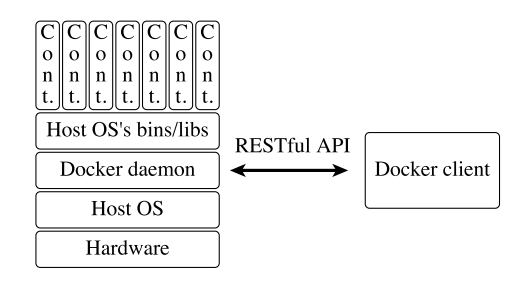
\includegraphics[width=\linewidth]{files/docker-engine.png} % Can you find an svg?
  \caption{Architecture of Docker engine \cite{bui2015analysis}}
  \label{figure-docker}
\end{figure}

Docker is an open-source container technology written in Go and launched in 2013 \cite[text]{docker-what}. The platform consists of the Docker Engine packaging tool, Docker image registries such as the Docker Hub public image repository and the Docker desktop application \cite{docker-overview}. In general, the engine architecture is similar to container-based virtualization, as visible in Figure~\ref{figure-docker} \cite{bui2015analysis}. The containers run on top of the Docker daemon, which manages and executes all the containers. The daemon is exposed to Docker clients via the RESTful HTTP API. The Docker client is a command-line tool which provides user interface for commanding the daemon, and thus containers. By exposing the API outside the host machine, the architecture enables remote control of the daemon with the client. Remote communication with the API should be carried out over TLS for security reasons.

Docker image is a read-only template with instructions for creating a Docker container \cite{docker-overview}. Images are often based on another image, such as OS images \texttt{ubuntu} and \texttt{alpine}, with some additional customizations, such as the installation of web server binaries. Customizations are added to the image as a series of data layers so that each new command creates a new layer. This process makes image distribution more efficient since only the changes between layers must be distributed \cite{bui2015analysis}. Layering is achieved with a special file system inspired by UnionFS that allows files and directories in different file systems to be combined into a single consistent file system.

Docker users can share their custom images publicly or privately in Docker Hub, or even host their own image registry platform. Most cloud providers also offer container registry services, so even proprietary software can be published in a private registry and used by other cloud services, like Kubernetes clusters. Whenever the image is not found locally, the client automatically attempts to search and pull the image from the connected registries.
\jb{Docker can only create and destroy containers. This makes it a runtime. This is an important concept to mention.}

\subsection{Kubernetes}

Kubernetes (K8s) \cite{kubernetes} is an open-source container orchestrator, i.e., a system to automate the deployment, scaling and management of containerized applications. It allows the creation of a cluster which consists of a set of servers, called Nodes, on which application containers are scheduled by the system. The automation provides resilience and efficient resource utilization for workloads in the cluster: if a container or Node dies, the system attempts to restart and reschedule containers so that the desired cluster state is maintained. K8s is hosted by the Cloud Native Computing Foundation (CNCF), but its origins are at Google, where it was created as an open-source option for Google's proprietary Borg and Omega orchestrators \cite{burns2016borg}. K8s was open-sourced in 2014.

\subsubsection{Kubernetes objects}

\textbf{Pods} are the basic atomic scheduling unit in K8s. Pods consist of one or more tightly-coupled containers with shared storage volume and networking \cite{k8s-docs-pods}. Containers in a Pod are always co-located and co-scheduled and run in a shared context, i.e. a set of Linux namespaces. The network, UTS and IPC namespaces are shared by default, and the process namespace can be shared with \texttt{v1.PodSpec.shareProcessNamespace}. The common network namespace means that containers in a Pod can communicate with each other via localhost, have a common IP address, and cannot reuse the same port numbers. In addition to the normal application container, Pods can include special \texttt{initContainers} that are run only on Pod startup. These Pods are used to modify the Pod context before the actual workload starts. Multiple \texttt{initContainers} are run sequentially, and a failing container blocks the execution of the following initialization and normal workloads.

If a Pod fails, a replacement Pod is not automatically created. Quite often, developers want to have more control over the compute resources and specify a target state for them. This includes replication, scaling, and distribution among various nodes. To meet these needs, K8s provides additional resources.

Instead of directly creating Pods, \textbf{Deployment} workload resources can be used to create Pods in a cluster \cite{k8s-docs-pods}. With Deployments, the user describes the desired state in a declarative manner. The Kubernetes control loop then creates \textbf{ReplicaSet} based on the Deployment resource, which in turn guarantees the availability of the desired number of Pods \cite{k8s-docs-deployment}. \textbf{DaemonSet} on the other hand is a workload resource that ensures that all or some Nodes run a copy of a Pod. Typical use cases for daemons are running Node monitoring and logging, and network plugins, which are discussed in depth in the Chapter~\ref{cni}.

All Pods across the cluster share the same subnet and can access each other via IP address. However, connecting to a Pod with IP address is suboptimal, since Pods are ephemeral. A dead Pod, even if controlled by a ReplicaSet, is not guaranteed to receive the same IP address on restart. Additionally, each replica in a horizontally scaled system has its own IP address. This leads to a problem: how do the clients using the system find and keep track of the IP addresses used by the workload? The \textbf{Service} abstraction solves the problem.

\textbf{Services} are an object for exposing groups of Pods over a network \cite{k8s-docs-services}. The object defines a set of endpoints, that is, the targeted Pods, along with a policy about how to make the Pods accessible. The targeted Pods are determined with a \texttt{selector} field in the object specification. Meanwhile, the \texttt{type} field determines how the Service is exposed. There are four different \texttt{ServiceTypes}: i) the default \texttt{ClusterIP} which exposes the Service inside the cluster with its own IP address, ii) \texttt{NodePort} which exposes the service in each Node's IP address on static port (by default within a range of 30000-32767), iii) \texttt{LoadBalancer} which exposes the Service externally using cloud provider's load balancer, and iv) \texttt{ExternalName} which is used to map Service to DNS name instead of a group of Pods. The field is designed as a nested functionality; each \texttt{ServiceType} level adds up to the previous one.

\jb{Usually services are proxies that route requests to the different Pods. There are also Headless services that only add DNS entries for the Pods.}

\textbf{Namespaces} allow logical grouping of resources under a single name. New K8s cluster starts with four namespaces: \texttt{default}, \texttt{kube-node-lease}, \texttt{kube-public} and \texttt{kube-system}. Namespaced objects like Deployments, Services and Pods are always deployed under a namespace which is \texttt{default} if not explicitly defined. \texttt{kube-system} is the namespace for all objects created by the K8s system which is discussed in more detail in the next Chapter~\ref{control-plane}. Namespaces also provide a scope for naming; names of resources need to be unique within a namespace, but not across namespaces. Namespaces are also used to enforce resource quotas, access control, and isolation for cluster users, for example, in multi-tenancy setups. Pod Security Standards \cite{k8s-docs-pss}, which are used by the Pod Security admission controller, are also defined at the namespace level. Admission controllers are discussed in Chapter~\ref{admission-controllers}.

\textbf{Custom Resource Definitions} (CRD) are used to define new resources that are not available in a default Kubernetes installation \cite{k8s-docs-crd}. Once a custom resource is installed, users can create and access custom resource objects with \texttt{kubectl}, similarly to any other built-in resource. On their own, custom resources can only be used to store and retrieve structured data. When combined with a custom controller, custom resources can be used to add new functionality to the cluster. In Kubernetes, controllers are a construct that watch the current state of the cluster and keep track of the desired state. If the states differ, the controller makes or requests changes so that the cluster state moves closer to the desired one. Specifically, the controllers are implemented as \textbf{Operators} following the \emph{operator-pattern} \cite{k8s-docs-operators}. The Operators are clients of the Kubernetes API that implement the control loop on a Custom Resource. They are often deployed as Deployments, and behave similarly to any other container workload in the cluster.

\subsubsection{Kubernetes components} \label{control-plane}

\begin{figure}[h!]
  \centering
  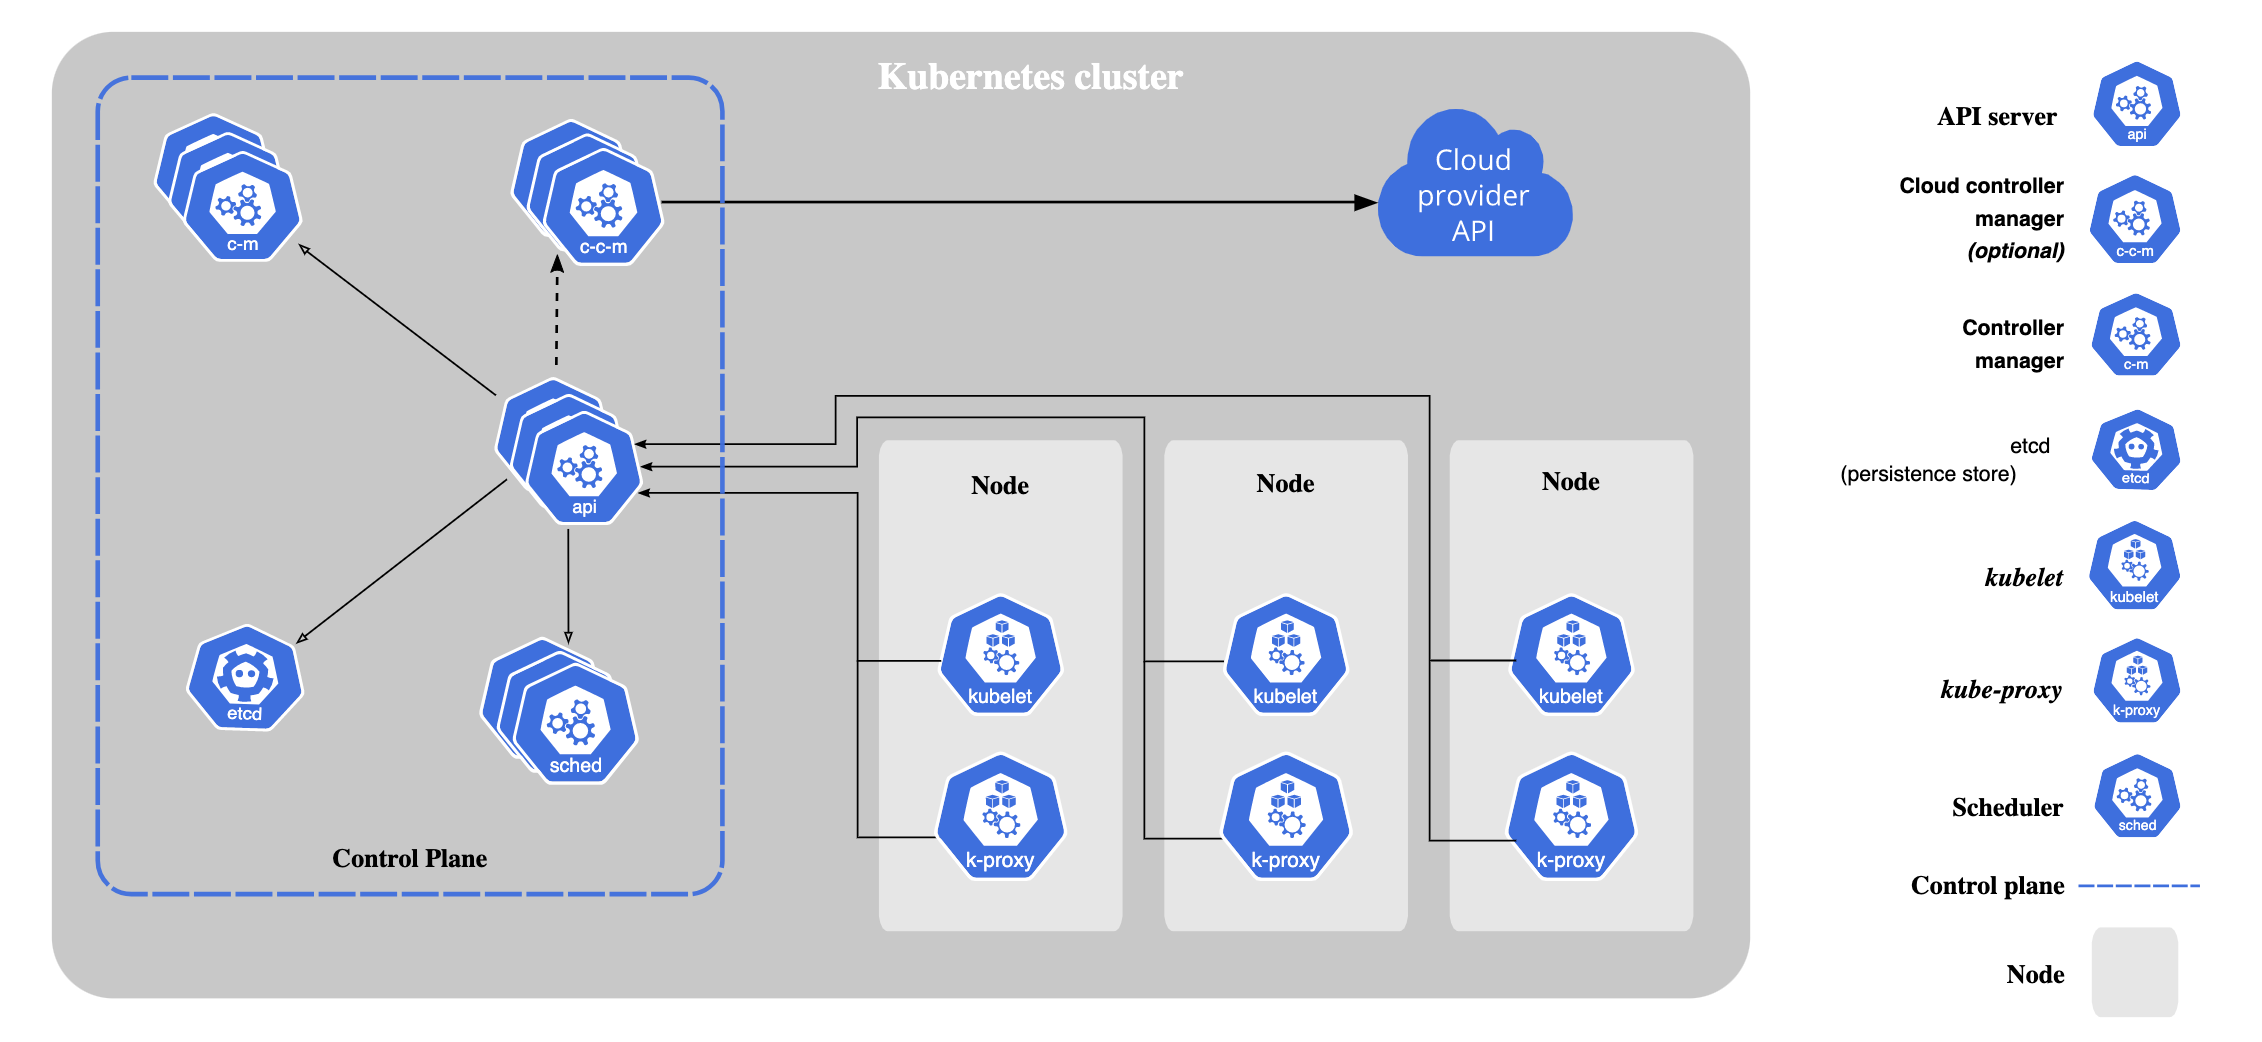
\includegraphics[width=\linewidth]{files/k8s-arch.png}
  \caption{Kubernetes cluster architecture \cite{k8s-docs-control-plane}}
  \label{figure-2}
\end{figure}

Figure~\ref{figure-2} describes the Kubernetes cluster with a control plane and three worker nodes. The control plane consists of components that control, monitor, and store the state of the cluster; essentially, these are the components that are needed for the complete and working Kubernetes cluster \cite{k8s-docs-control-plane}. The control plane components can run on any worker node. However, clusters often have a specialized master node for control plane components, which does not run any other containers. For fault tolerance and high availability, control plane components should run on multiple Nodes in production environments. The control plane consists of these main components:

\textbf{API server} is a front-end component of the control plane. It is an HTTP server that is used to send commands to the cluster. The server handles authentication and validation of the commands. For valid commands, the server then forwards these to other control plane components that then modify the cluster state. The easiest way to send commands to the server is by using the \texttt{kubectl} command-line interface (CLI) tool, which actively sends the commands as HTTP under the hood. The main implementation of the server is \texttt{kube-apiserver}. The server can be horizontally scaled by running several instances on multiple Nodes and load-balancing traffic between the instances.

\textbf{Etcd} \cite{etcd} is a highly consistent, distributed key-value store. It is the stateful component of the control plane: all of the cluster data is stored in etcd. Thus, the stability of the component is critical for the whole cluster. To tolerate failures, etcd implements a leader-based architecture. Multiple etcd clients automatically elect a leader instance as the source of truth. Other instances periodically update their state from the leader instance, so that the state stays eventually consistent across all instances. On leader failure, the other instances automatically elect a new leader to keep the system functioning.

\textbf{Scheduler} watches for newly created Pods that have no assigned worker node, and selects one of the active Nodes for them to run on \cite{k8s-docs-control-plane}. Scheduling takes into account resource availability on Nodes, Pod resource requirements, object specification affinity rules and hardware, software, and policy constraints, among others.

\textbf{Controller manager} is a control plane component that runs all the controller loop processes \cite{k8s-docs-control-plane}. Controller loops, like the Deployment controller, continuously watch the current and desired cluster state. When the states differ, they send commands via the API server so that the cluster moves towards the desired state. All the built-in controllers are compiled into a single binary, even though the controllers are logically different processes.

Each Node also has components that are essential for Kubernetes to work properly. \textbf{Kubelet} is an agent that ensures that containers are running in a Pod \cite{k8s-docs-control-plane}. It receives a set of Pod specification from the API server and ensures that containers are running on the Node, follow the Pod specifications and are healthy. \texttt{Kubelet} only manages containers created by Kubernetes. \textbf{Kube-proxy} maintains network rules on Nodes. Part of the Serivce objects' networking is implemented by \textbf{kube-proxy}; the proxy writes \texttt{iptables} rules that route traffic \cite{cilium-proxy-free}.

\subsubsection{Admission controllers} \label{admission-controllers}

Admission controllers are a feature of the Kubernetes API server, used to validate and modify requests made to the server \cite{k8s-docs-admission}. The controllers execute before the request is executed but after it is authenticated and authorized by the server. Several important features of Kubernetes are implemented with admission controllers, and these should be enabled on a properly configured API server. In addition to the built-in controllers, Kubernetes provides \texttt{MutatingAdmissionWebhook} and \texttt{ValidatingAdmissionWebhook} controllers for building own admission logic.

Admission controllers can be validating, mutating, or both \cite{k8s-docs-admission}. Mutating controllers may modify related objects to the requests they admit, while validating controllers either approve or reject the request. The control process first executes the mutating controllers so that no mutations occur after the validation. If a controller in either phase rejects the request, the request is not processed further, and error is returned to the end-user.

One notable Admission controller is the \texttt{PodSecurity} controller. The controller validates the Pods before they are admitted, making sure that the requested Pod security context and other restrictions are permitted in the namespace to which the Pod is assigned \cite{k8s-docs-admission}. The controller is enabled by default, and can be taken into use just by configuring Pod Security Admission labels for Namespace objects.

The labels use \texttt{pod-security.kubernetes.io/<MODE>: <LEVEL>} format, where MODE defines the action to be taken when the security level is violated and LEVEL is a predefined level of the Pod Security Standard. The three available levels are \texttt{privileged}, \texttt{baseline} and \texttt{restricted} \cite{k8s-docs-pss}.

The available actions are i) \texttt{enforce}, which will reject the Pod on violation, ii) \texttt{audit}, which triggers an event about the violation in the audit log, and iii) \texttt{warn}, which triggers user-facing warning about the violation \cite{k8s-docs-psa}. A namespace can configure any or all three of the available modes and even set a different level for the modes. For example, it is possible to warn the user about violation of security policies without blocking the request by setting the \texttt{warn} mode more restrictive than \texttt{enforce}.

% https://learn.microsoft.com/en-us/azure/architecture/patterns/sidecar
\subsubsection{Sidecar pattern in Kubernetes}

As mentioned before, Pods are the basic scheduling abstraction in Kubernetes and they support management and co-scheduling of multiple containers as an atomic unit.
This co-scheduling and management of multiple symbiotic containers as a single unit enables multi-container application design patterns to emerge \cite{burns2016design}.
The sidecar pattern is the most common of these design patterns.
As an example of this pattern, the main application container can be a simple web server paired with a container that collects server logs from a file and streams them to a centralized log management system.
Listing~\ref{lst:sidecar-pattern} shows how the logs can be shared to the sidecar with file mounts.
Another example of this pattern is the Istio service mesh \cite{istio} and its Envoy proxy sidecar, which routes all traffic through the Istio control plane for management, observability, and security operations.

\lstinputlisting[
  caption={Nginx web server with a sidecar that periodically reads the logs},
  label={lst:sidecar-pattern},
  language=yaml
]{code/sidecar-pattern.yml}

% First, the container is the unit of resource accounting and allocation, so for example a web server container’s cgroup can be configured so that it provides consistent lowlatency responses to queries, while the logsaver container is configured to scavenge spare CPU cycles when the web server is not busy. Second, the container is the unit of packaging, so separating serving and log saving into different containers makes it easy to divide responsibility for their development between two separate programming teams, and allows them to be tested independently as well as together. Third, the container is the unit of reuse, so sidecar containers can be paired with numerous different “main” containers (e.g. a log saver container could be used with any component that produces logs). Fourth, the container provides a failure containment boundary, making it possible for the overall system to degrade gracefully (for example, the web server can continue serving even if the log saver has failed). Lastly, the container is the unit of deployment, which allows each piece of functionality to be upgraded and, when necessary, rolled back, independently. (Though it should be noted that this last benefit also comes with a downside – the test matrix for the overall system must consider all of the container version combinations that might be seen in production, which can be large since sets of containers generally can’t be upgraded atomically. Of course while a monolithic application doesn’t have this issue, componentized systems are easier to test in some regards, since they are built from smaller units that can be independently tested.) Note that these five benefits apply to all of the container patterns we describe in the remainder of this paper.

In the pattern, peripheral tasks such as logging, configuration, and observability are isolated from the main application into helper containers.
These containers, sidecars, are tightly-coupled to the parent application container and should share the lifecycle of the parent.
Although sidecar functionality could be built into the main container, there are benefits in using separate containers \cite{burns2016design}.
The isolation allows tweaking of containers' cgroups so that CPU cycles can be prioritized for the main container.
The isolation also provides a failure containment boundary between the main and sidecar processes.
Since the container is also the unit of deployment, sidecar containers could be developed, tested, and deployed independently of each other.
Sidecar containers can also be developed with different tools and dependencies and in a way that they can be reused with other application containers.
From the testing point of view, the componentized system might improve testing if the smaller units can be tested independently.
However, on the downside, the combination of all container version combinations that might be seen in a production environment also increases.

\subsection{Kubernetes network model}

% https://kubernetes.io/docs/concepts/services-networking/
% https://kubernetes.io/docs/concepts/extend-kubernetes/compute-storage-net/network-plugins/

% The key requirements of the Kubernetes network model include i) Pods are IP addressable and must be able to communicate with all other Pods (on the same or different host) without the need for network address translation (NAT), and ii) all the agents on a host (e.g., Kubelet) are able to communicate with all the Pods on that host. CNI plugins may differ in their architecture but meet the above network rules.

A fundamental part of a Kubernetes cluster is how nodes and resources are networked together. Specifically, the networking model needs to address four different types of networking problems: i) intra-Pod (that is, container-to-container within the same Pod) communication, ii) inter-Pod communication between Pods, iii) Service-to-Pod communication and iv) communication from external sources to Services \cite{k8s-docs-cluster-networking}. The model also requires that each Pod is IP addressable and can communicate with other Pods without network address translation (NAT), even when Pods are scheduled on different hosts \cite{qi2020assessing}. All agents on a host should also be able to communicate with Pods on the same host. The implementation of this model is not part of Kubernetes, but is handed to special plugins that implement the Container Network Interface (CNI) specification.
\jb{K8s defines the CNI interface to allow different vendors and operators to use different networking mechanisms in kubernetes.}

\subsubsection{Container Network Interface} \label{cni}

The Container Network Interface (CNI) \cite{cni} is a networking specification, which has become the de-facto industry standard for container networking. It is backed by CNCF \cite{qi2020assessing}. CNI was first developed for the container runtime \texttt{rkt} \cite{hausenblas2018container}, but it is supported by all container runtimes, and there are a large number of implementations to choose from. Most container orchestrators have adopted the specification as their networking solution. The biggest outlier is Docker Swarm, which instead implements its own proprietary approach to container networking.

The CNI specification has five distinct definitions: i) a format for network configuration, ii) an execution protocol between the container runtimes and the plugin binary, iii) a procedure for the runtime to interpret the configuration and execute the plugins, iv) a procedure for delegating functionality between the plugins, and v) data types for the plugins to return their results to the runtime \cite{cni}. The network configuration is defined as a JSON file, and it includes a list of plugins and their configuration. The container runtime interprets the configuration file at the plugin execution time and transforms it into a form to be passed to the plugins. The execution protocol defines a set of operations (ADD, DEL, CHECK, VERSION) for adding and removing containers from the network. The operation command, similarly to other protocol parameters, is passed to the plugins via the OS environment variables. The configuration file is supplied to the plugin via stdin. On successful execution, the plugin returns the result via stdout with a return code of 0. On errors, the plugin returns a specific JSON structure error message to stderr and a non-zero return code. When runtime mutates a container network, it results in a series of ADD, DELETE, or CHECK executions. These are then executed in the same order as defined in the \texttt{plugins} list, or reversed order for DELETE executions. Each plugin then returns either \texttt{Success} or \texttt{Error} JSON object. The execution of a series of operations ends when it encounters the first error response, or when all the operations have been performed.

% When a new Pod is added, the CNI plugin coordinates with the container runtime and connects the container network namespace with the host network namespace (e.g., , veth pair), assigns a unique IP address to the new Pod, applies the desired network policies and distributes routing information to the rest of the cluster.

% https://www.tkng.io/cni/

% Connectivity - making sure that a Pod gets its default eth0 interface with IP reachable from the root network namespace of the hosting Node.
% Reachability - making sure that Pods from other Nodes can reach each other directly (without NAT).

% Connectivity requirement is the most straight-forward one to understand – every Pod must have a NIC to communicate with anything outside of its own network namespace. Some local processes on the Node (e.g. kubelet) need to reach PodIP from the root network namespace (e.g. to perform health and readiness checks), hence the root NS connectivity requirement.

% Reachability, on the other hand, may require a bit of unpacking:
% - Every Pod gets a unique IP from a PodCIDR range configured on the Node.
% - This range is assigned to the Node during kubelet bootstrapping phase.
% - Nodes are not aware of PodCIDRs assigned to other Nodes, allocations are normally managed by the controller-manager based on the --cluster-cidr configuration flag.
% - Depending on the type of underlying connectivity, establishing end-to-end reachability between PodCIDRs may require different methods:
%   - If all Nodes are in the same Layer2 domain, the connectivity can be established by configuring a full mesh of static routes on all Nodes with NextHop set to the internal IP of the peer Nodes.
%   - If some Nodes are in different Layer2 domains, the connectivity can be established with either:
%     - Orchestrating the underlay – usually done with BGP for on-prem or some form of dynamically-provisioned static routes for public cloud environments.
%     - Encapsulating in the overlay – VXLAN is still the most popular encap type.

The CNI plugin must provide at least connectivity and reachability for the containers \cite{cni-tkng}.
For connectivity, each Pod must have a network interface controller (NIC) for communication outside its networking namespace.
The NIC must have an IP address that is reachable from the host Node, so that cluster processes like Kubelet health and readiness checks can reach the Pod.

Reachability means that all Pods can be reached from other Nodes directly without NAT.
Thus, each Pod should receive a unique IP address from an IP pool range designated for the Pods.
When a cluster is installed, the administrator assigns a CIDR for the whole cluster.
Then the \texttt{kube-controller-manager} can be configured to assign each node its own CIDR range, defined in the Node's \texttt{spec.podCIDR} field.
The IP addresses are assigned to the Pods by an IP address management (IPAM) plugin.
IPAM plugins are \emph{delegated plugins} of the CNI, which means that the CNI plugin is responsible for invoking the IPAM plugin when needed.
Thus, many CNI plugins are installed with their own IPAM plugins for convenience.
Quite often IPAM plugins assign Pods with IP address from the Node's \texttt{podCIDR}, but sophisticated IPAMs like those of Calico and Cilium use Custom Resources for more configurable IP pools.
The end-to-end reachability between different Node \texttt{PodCIDR}s is established by encapsulating in the overlay network, for example, with Virtual Extensible LAN (VXLAN), or orchestrating on the underlay network, e.g. with Border Gateway Protocol (BGP).

% Kubernetes Network Policy is the means to enforce rules
% indicating which network traffic is allowed and which Pods
% can communicate with each other. The policies applied to Pod
% network traffic can be based on their applicability to ingress
% traffic (entering the Pod) and egress traffic (outgoing traffic).
% The control strategies include “allow” and “deny”. By default,
% a Pod is in a non-isolated state. Once a network policy is
% applied to a Pod, all traffic that is not explicitly allowed will
% be rejected by the network policy. However, other Pods that do
% not have network policies applied to them are not affected. CNI
% plugins in Kubernetes can implement elaborate traffic control
% and isolation mechanisms.

% Network policies help to provide the guardrails needed to
% restrict traffic between Pods (in and/or across namepaces) as
% well as between Pods and external networks, by explicitly
% specifying allowed and denied connections. A network policy
% specification consists of a podSelector to specify Pods
% that will be subject to the policy and policyTypes to
% specify the types of policies, i.e., ingress and/or egress. Ingress
% rules specify allowed inbound traffic to the target Pods, and
% egress rules specify allowed outbound traffic from the target
% Pods. Each rule is comprised of a NetworkPolicyPeer
% for selecting Pods on the other side of the connection to/from
% which traffic is allowed, through a Classless Inter-Domain
% Routing (CIDR) notation that specifies IP address blocks,
% namespaces, or Pod labels; and a NetworkPolicyPort
% that allows to explicitly specify ports or protocols that may
% communicate with the Pod. Network policies are additive, and
% if multiple policies select a Pod, traffic is restricted to what is
% allowed by the union of those policies’ ingress/egress rules.

Since Kubernetes does not provide networking between Pods, it has no capabilities to enforce network isolation between workloads.
Thus, another key feature of some CNI plugins is the enforcement of network traffic rules.
For this purpose, Kubernetes provides a common built-in resource called \texttt{NetworkPolicy} for the CNI plugins to consume.
The Listing~\ref{lst:example-np} is an example of network policies for a web application front-end.
The first policy functions as a default rule that denies all implicit egress and ingress traffic.
The second policy allows traffic to the default HTTP port, and the third policy allows the front-end application to send traffic to any Pod in the \emph{backend} namespace.

\lstinputlisting[
  caption={Example NetworkPolicies for a frontend web application},
  label={lst:example-np},
  language=yaml
]{code/example-network-policy.yml}

The NetworkPolicy specification consists of a \texttt{podSelector} that specifies Pods that are subject to the policy and \texttt{policyTypes} to specify the Ingress and Egress rules for the traffic \cite{budigiri2021network} to the target Pod. Each rule includes \texttt{to} or \texttt{from} field for selecting Pod, Namespace or IP address block in CIDR notation on the other side of the connection, and \texttt{ports} field for explicitly specifying which ports and protocols are part of the rule. The policies are additive; when multiple rules are defined for a Pod, the traffic is restricted to what is allowed by the union of the policies. Many CNI plugins also introduce Custom Resource Definitions for their own, more granular, network policy rules.

% TODO: Not everything listed above is requirements
Although all CNI plugins meet the requirements listed above, they may differ in architecture significantly. The plugins can be classified based on which OSI model network layers they operate on, which Linux kernel features they use for packet filtering and which encapsulation and routing model they support for inter-host and intra-host communication between Pods. In this thesis, we focus on three different CNI plugins: Calico, Cilium, and Multus.

% TODO: CNI plugins, daemons and binary \cite{qi2020understanding}.

% Src: https://www.youtube.com/watch?v=0jJBUdYOmRU
% Configurations in /etc/cni/net.d on nodes
% Kubelet monitors the directory, no need to restart it when installing CNI

\subsubsection{Calico}

Calico \cite{calico} is an open-source CNI plugin with modular architecture that supports a wide range of deployment options. Each Pod created in the Calico network receives one end of a virtual ethernet device link as its default \texttt{eth0} network interface, while the other end is left dangling on the host Node \cite{calico-tkng}. The Pod end of the link receives an IP address from Pod CIDR, but the Node end does not. Instead, a \texttt{proxy\_arp} flag is set on the host side of the interface, while containers have a route to link-local address \texttt{169.254.1.1}, thus making the host behave like a gateway router. For routing packets between Nodes, Calico creates a VXLAN overlay network. Optionally, Calico supports IP-in-IP overlay or non-overlay network with BGP protocol.

On each Node, a \texttt{calico-node} daemon setups CNI plugin, IPAM, and possible eBPF programs. The daemon subscribes to Kubernetes API for Pod events and manages both container and host networking namespaces. Calico also deploys a single-container \texttt{calico-kube-controllers} Pod into the Kubernetes control plane. The container executes a binary that consists of controller loops for Namespace, NetworkPolicy, Node, Pod, and ServiceAccount Kubernetes objects. The Calico project also introduces its own CLI tool, called \texttt{calicoctl} \cite{calicoctl}, to manage Calico's custom resources. The tool provides extra validation for the resources which is not possible with \texttt{kubectl}.

Calico supports Kubernetes NetworkPolicies as well as its own namespaced \\\texttt{projectcalico.org/v3.NetworkPolicy} Custom Resource Definition. Both of the policies work on OSI layers L3 (identity, e.g. IP address) and L4 (ports). Compared to the built-in policy, the Calico policy includes features such as policy ordering, log action in rules, and more flexible matching criteria (e.g., mathcing on ServiceAccounts) \cite{calico-network-policy}. The policy can also match other Calico CRDs such as \textbf{HostEndpoints} and \textbf{NetworkSets}, which allows implementing rules on host interfaces and non-Kubernetes resources. If Calico is installed along the Istio service mesh, the Calico Network Policy can enforce L7 (e.g. HTTP methods and URL paths) policies on the Envoy proxy. For policies that are not tied to a Kubernetes namespace, Calico provides a \texttt{GlobalNetworkPolicy} CRD.

\jb{Now that Calico uses eBPF there is little difference between them and both can reduce the amount of sidecars to one per node.}

\subsubsection{Cilium}

Cilium \cite{cilium} is one of the most advanced and powerful CNI plugins for Kubernetes. Similarly to Calico, it creates a virtual ethernet device for each Pod and sets one side of the link into the Pod's network namespace \cite{cilium-tkng} as the default interface. Cilium then attaches extended Berkeley Packet Filter (eBPF) programs to ingress traffic control (\texttt{tc}) hooks of these virtual ethernet devices to intercept all incoming packets from the Pod. The packets are intercepted and processed before the network stack, and thus \texttt{iptables}, reducing latency 20\%-30\% and even doubling the throughput of packets in some scenarios \cite{budigiri2021network}. The network between Pods running on different hosts is handled by default with VXLAN overlay, but there is support for Geneve interfaces and native-routing with the BGP protocol as well \cite{cilium}.

The Cilium system consists of an agent (\texttt{cilium-agent}) daemon running on each Node, one or more operator (\texttt{cilium-operator}) Pods and a CLI client (\texttt{cilium}) \cite{cilium-components}. The agent daemons subscribe to events from the Kubernetes API and manage containers' networking and eBPF programs. The CLI tool, which is installed on each agent, interacts with the REST API of the agent and allows one to inspect the state and status of the local agent. The tool should not be confused with the Cilium management CLI tool, also incidentally named \texttt{cilium}, which is typically installed remote from the cluster. The operator is responsible for all management operations that should be handled once for the entire cluster, rather than once for each Node. This includes, for example, the registration of CRDs.

% TODO: Move OSI layer to somewhere else
Although default Kubernetes NetworkPolicies provides security on OSI layers L3 and L4, Cilium provides CRDs that also support L7 policies \cite{cilium-policy-language}. If L7 policies exist, the traffic is directed to Envoy instance bundled into the agent Pod which filters the traffic. Unlike on layers 3 and 4, policy violation does not result in dropped packet but an application protocol specific denied message. For example, HTTP traffic is denied with \texttt{HTTP 403 Forbidden} and DNS requests with \texttt{DNS REFUSED}. Cilium provides \texttt{CiliumNetworkPolicy} CRD that supports all L3, L4, and L7 policies. Cilium also provides \texttt{CiliumClusterwideNetworkPolicy} custom resource which is used to apply network rules to all namespaces in the cluster or even to nodes when using \texttt{nodeSelector}.

As even more advanced features, Cilium also includes natively \texttt{kube-proxy} replacement, encryption for Cilium-managed traffic, and Service Mesh, among others. By default, \texttt{kube-proxy} uses \texttt{iptables} to route the Service traffic \cite{cilium-proxy-free}. With \texttt{kubeProxyReplacement} installation option, Cilium implements Service load-balancing as XDP and TC programs on the Node network stack. For encryption, Cilium supports IPsec and WireGuard implementations \cite{cilium-encryption}. The service mesh performs a variety of features directly in eBPF, thus functioning without sidecar containers or proxying requests through the agent Pod's Envoy \cite{cilium-service-mesh}. Since all features are not available as eBPF programs or on all kernel versions,  Cilium automatically probes the underlying kernel and automatically reverts to the Envoy proxy when needed. For capabilities beyond the built-in mesh, Cilium also provides integration with Istio.

\jb{Have you thought about how your solution is impacted by eBPF?}
% \begin{itemize}
  % \item More on network rules (probes and uses most recent features from Kernel)
  % \item Transparent encryption https://docs.cilium.io/en/v1.13/security/threat-model/
  % \item Security on different levels: https://docs.cilium.io/en/v1.13/security/network/intro/
  % \item Cilium Service Mesh https://isovalent.com/blog/post/cilium-service-mesh/
  % \item Kube-proxy replacement
  % \item Cilium components (Agent (includes Envoy), client, operator, plugin). Hubble?
% \end{itemize}

\subsubsection{Multus}

Traditionally, CNI plugins provide only a single network interface for a Pod, apart from the loopback device. Multus \cite{multus-cni} is a CNI plugin that allows the attachment of multiple network interfaces for a Pod. It does not provide any connectivity or reachability for containers like other plugins. Instead, it is installed as the first plugin in the CNI plugin chain. When executed, the plugin delegates the creation of the interface to other installed plugins. Since Multus does not provide any networking and thus does not independently, it is often called \emph{meta plugin} to distinguish it from common CNI plugins like the previous Calico and Cilium.

Multus system includes a binary, a CNI configuration file, and a namespaced \texttt{NetworkAttachmentDefinition} CRD that is used to define network interfaces used in Pods. The binary and the configuration file are often installed on cluster nodes via a DaemonSet. The daemon consists of an \textit{initContainer} that copies the binary into the \texttt{/opt/cni/bin} directory, and a daemon container that configures the configuration file and optionally spawns an HTTP server for additional features such as metrics \cite{multus-cni}. The configuration file satisfies the CNI specification with few additional attributes of which the combination of \texttt{clusterNetwork} and \texttt{defaultNetworks} or \texttt{delegates} are imperative for the CNI plugin to function \cite{multus-cni-config}. The \texttt{clusterNetwork} specifies the main network of the cluster, which implements the \texttt{eth0} interface and the Pod IP address. The \texttt{defaultNetworks} is an optional array of networks that should be added for any Pods by default. The values can be names of the \texttt{NetworkAttachmentDefinition} objects or paths to the CNI plugin's JSON configuration files. Optionally, the \texttt{delegates} attribute can be used; it supports similar format of values. In this scenario, the first element of the array functions as \texttt{clusterNetwork} and the rest are inferred as \texttt{defaultNetworks}.

% TODO: Add examples of NetworkAttachmentDefinition and Pod annotations

Attaching additional interfaces to workloads is most often configured by adding a special annotations field \texttt{k8s.v1.cni.cncf.io/networks} to workload resource definitions. In the simplest configuration, the field takes a comma separated list of the \texttt{ NetworkAttachmentDefinition} names as input. The network interface identifiers can be modified by providing the attachment input in \textit{name@interface-identifier} format. Otherwise, Multus names the interfaces \textit{net0}, \textit{net1} and so on. If extra configuration for the networks is needed, the annotation also supports the JSON array format.

\subsubsection{Extended Berkeley Packet Filter}

Berkeley Packet Filter (BPF, or nowadays often cBPF) was originally developed in the early 1990s as a high-performance tool for user-space packet capture \cite{mccanne1993bsd}. BPF works by deploying the filtering part of the application, \texttt{packet filter}, in the kernel-space as an agent. The \texttt{packet filter} is provided with a program (often denoted as BPF program) consisting of BPF instructions, which works as a set of rules for selecting which packets are of interest in the user-space application and should be copied from kernel-space to user-space. The instructions are executed in a register-based pseudo machine. Since network monitors are often interested only in subset of network traffic, this limits the number of expensive copy operations across the kernel/user-space protection boundary only to packets that are of interest in the user-space application. A notable use-case for BPF is \textit{libpcap} library, which is used by a network monitoring tool called \texttt{tcpdump}.

Later in the 2010s the Linux community realized that BPF and it's ability to instrument the kernel could benefit other areas than packet filtering as well \cite{vieira2020fast}. This reworked version of BPF was first merged into the Linux kernel in 2014 and is publicly called the extended Berkeley Packet Filter (eBPF) to distinguish it from the original cBPF. The kernel development community continues to call the newer version BPF, but instead of the original acronym consider it a name of a technology. Similarly to the kernel community, the term BPF always refers to the eBPF in this thesis.

The eBPF programs are compiled to bytecode and loaded into the kernel with \texttt{bpf()} system call \cite{miano2021framework}. Most often, programs are written in restricted C and compiled with the LLVM Clang compiler to bytecode. It is also possible to use the eBPF assembly instructions and \texttt{bpf\_asm} utility for converting instructions to bytecode. eBPF programs follow an event-driven architecture: a loaded eBPF program is hooked to a particular type of event, and each occurrence of the event triggers the program execution.

There are two different network event interfaces in eBPF: eXpress Data Path (XDP) and Traffic Control (TC) \cite{miano2021framework}.
XDP programs are attached to an NIC and can handle only incoming packets \cite{hoiland2018express}. The programs are called directly by the NIC driver if it has XDP support, thus executing before packets enter the network stack. This skips expensive packet parsing and memory allocation operations and allows XDP programs to run at very high throughput. Thus, even the main network buffer \textit{skbuff} is not populated. Some SmartNICs even support offloading the program to the NIC's own processor from the host CPU, further improving the performance of the host machine \cite{cilium-program-types}. If the driver does not support XDP, generic XDP is used and the programs run after the packet has been parsed by the network stack.

% In Cloudflares DDoS testing benchmark \cite{cloudflare-xdp}, XDP program was capable to drop 10 million and TC program 2 million packets per second, while common \texttt{iptables} INPUT rule was able to drop less than one million packets per second.

XDP programs can read and modify the contents of packets \cite{vieira2020fast}. Since the packets are not parsed into the network stack, the programs have to work with raw packets and implement their own parsing functionality. The program's return value determines how the packet should be processed further. With \texttt{XDP\_DROP} and \texttt{XDP\_PASS} return values, the packet can be dropped or passed further to the networking stack, respectively. The packet can also be bounced back to the same NIC on which it arrived with \texttt{XDP\_TX}, usually after modifying the contents of the packet. \texttt{XDP\_REDIRECT} is used for redirecting the packet to a different NIC, CPU or even to another socket.

TC programs are executed when both incoming and outgoing packets reach the kernel traffic control function within the Linux network stack \cite{vieira2020fast}. The ingress hook runs after the packet is parsed to \textit{skbuff} but before most of the network stack. On egress the stack is traversed in reverse; thus, the hook executes after most of the network stack. TC programs can read and write directly to a packet in memory. Similarly to XDP programs, the return value of the program determines the further processing of the packet. The packet can be passed further in the stack with \texttt{TC\_ACT\_OK}, dropped with \texttt{TC\_ACT\_SHOT}, or the modified packet can be redirected back to the start of the classification with \texttt{TC\_ACT\_RECLASSIFY}, among others.
\jb{Do we need this level of detail to understand your solution?}
% TODO: delete or find a good place for these scenarios
\clearpage
\subsection{Example attack scenarios}
\jb{This is part of the threat modeling}

\begin{itemize}
  \item Privileged container
  \item CAP\_SYS\_ADMIN, mounting /proc and chroot
  \item CAP\_SYS\_PTRACE, shellcode injection to running program, nc 172.17.0.1 on port running shell
  \item Mounted docker socket, creating privileged containers
\end{itemize}

All of the example attack scenarios start by an attacker getting shell access to a container running in a Pod, usually through a remote code execution (RCE) flaw on the container application and then executing reverse shell inside the Pod. The scope of the examples is not in the initial attack, but in the Pod template misconfigurations that then provide some path for the attacker to escalate the attack and even take over the whole cluster in the end.

TODO: add file \label{yaml:priv-container}

The first attack scenario includes a privileged container, as described in File~\ref{yaml:priv-container}. Privileged containers have all the capabilities of the host machine, so practically they can be perform almost any action available on the host. This includes, but is not restricted to, for example "pipeing" (TODO: a better word for undock.sh and other scripts) commands as root to the Node's shell and mounting the host's disks. If combined with \texttt{hostPID:\ true}, the attacker can see all processes on the host and use \texttt{nsenter} to execute commands in the namespaces of the other processes.

TODO: add file \label{yaml:host-path}

The second example file~\ref{yaml:host-path} does not have similar privileges for executing commands as the first, but has unlimited access to mount the entire host's filesystem, with read and write access. Thus, the attacker can try to find any credentials stored on the host machine and use these to escalate the attack. Important credentials include \texttt{kubeconfig} files that store access tokens to the K8s API server, ServiceAccount tokens that may have been mounted on any Pod on the host, SSH keys and hashed user passwords in \texttt{/etc/shadows}.

TODO: some extra issues (finding .kubeconfig files, running on control-plane -> etcd and secrets within, cloud metadata)

\clearpage

\section{Solution requirements} \label{sec:methods}

\jb{Threat model can also be a separate section. In principle, you should discuss the attacks you want to defend against (e.g., installing a malicious sidecar, or legitimate sidecar with vulnerabilities), the location of the attacker in the system (inside a specific container, in any container, outside the cluster),
the prerequisites for an attack, and which parts of the threat matrix are involved.}



This chapter analyzes threats in the K8s cluster from the perspective of sidecars and defines the security requirements for the solution introduced in the following chapters. First, threat modeling is used to identify possible attack vectors and readily available mitigations. Then, the model is used to identify all issues that should be solved with the solution. Finally, an example development environment is introduced to test out the solution.

\subsection{Threat modeling}

% Threat modeling is a structured approach of identifying and prioritizing potential threats to a system, and determining the value that potential mitigations would have in reducing or neutralizing those threats

% Threat modeling methods are used to create an abstraction of the system; profiles of potential attackers, including their goals and methods; and a catalog of potential threats that may arise. There are many threat modeling methods that have been developed. Not all of them are comprehensive; some focus on the abstraction and encourage granularity while others are more people-centric. Some methods focus specifically on risk or privacy concerns. Threat modeling methods can be combined to create a more robust and well-rounded view of potential threats.

% A threat is defined as a potential loss of confidentiality and integrity of an asset caused by an attacker acting to compromise that asset via some attack surface.

A security threat is any possible event in a system that could lead to a potential loss of confidentiality and integrity of an asset in the system. Threat modeling is a structured approach to identify and prioritize potential threats to a system. This includes profiles of potential attackers and their goals and methods, as well as potential mitigations \cite{shevchenko2018threat}. The idea is to build a catalog of all potential threats, prioritize issues and try to find mitigations so that attackers cannot use the vulnerabilities against the system.

% TODO: Check the NSA security stuff \cite{nsa-cisa-hardening}

For generic K8s clusters there exist a number of extensive threat models, for example the \textit{Threat Matrix for Kubernetes} by Microsoft \cite{k8s-threat-matrix}. The scope of this thesis is on sidecar security, so we will only focus on the possible threats that can be leveraged after the attacker has gained access to a sidecar container inside the cluster. The \textit{Threat Matrix for Kubernetes} is used to identify threats in this scenario, while the results are listed in Table~\ref{table:threat-model}.

\begin{table}[H]
  \sffamily% change the font in the table to sans serif
  \centering

  \caption{K8s sidecar threat model}
  \label{table:threat-model}

  % minipage so that footnotes are printed
  \begin{minipage}{\textwidth}
  % footnotes in minipage are letters instead of numbers, fix that
  \renewcommand{\thempfootnote}{\arabic{mpfootnote}}
  \begin{tabularx}{\textwidth}{CCC}
    \hline
    \textbf{Threat} & \textbf{Description} & \textbf{Mitigation}\\ \hline
    Privileged containers & If containers are given privileges, malicious actor can breakout from the container and escalate the attack on cluster. & Use \texttt{restricted} Pod Security Admission to enforce security rules. PSAs are defined for namespaces, so isolate privileged containers into their own namespaces to follow the principle of least privilege. \\ \hline
    Writing to the host file system & TODO. & Do not allow unnecessary mounts. Use \texttt{readOnlyRootFilesystem: true} whenever possible. \\ \hline
    Permissive RBAC on service accounts & Containers in a Pod share service accounts\footnote{\texttt{spec.serviceAccountName} is a Pod-level field}. By default, Pods automatically mount the service account to all containers. & Disable automatic mounting of service accounts\footnote{Set \texttt{automountServiceAccountToken: false}} and explicitly mount them to containers when needed. Adhere to the principle of least privilege. \\ \hline
    There are no resource limits for containers & If not set, a single container can hog system resources, causing denial of service (DoS). & Set resource limits to containers\footnote{Use \texttt{spec.containers[*].resources}}. \\ \hline
    The Pod has network access to the control plane & By default, all traffic inside the cluster is allowed. & Use NetworkPolicies as a firewall. Deny by default and explicitly allow traffic only if needed. \\ \hline
    Sidecar can use the main container's NetworkPolicy to access \texttt{kube-system} or other Pods & NetworkPolicies affect the NIC of the Pod network, which is shared by sidecars. & \textbf{No built-in solution available!} \\ \hline
    Sidecar has network access to cloud resources & Cloud providers may attach cloud identities to cluster Nodes, so that Pods can access resources outside the cluster. & \textbf{Same issue as above!} Block mounting volumes with access to cloud credentials. \\ \hline
    Sidecar has network access to the main container & Main container is accessible via loopback device, which cannot be protected with NetworkPolicy. & \textbf{There is no built-in solution available!} \\ \hline
    Sidecar is used to sniff the main application's traffic & TODO & mTLS? Requires a service mesh. \\ \hline
    Unencrypted secrets & TODO & Encrypt at rest \\ \hline
  \end{tabularx}
\end{minipage}
\end{table}


\subsection{Security requirements}

Threat modeling identified two main categories of issues: permissive workload configurations and networking related issues. Essentially, all the threats are caused by sidecars not respecting the principle of least privilege; the sidecar inherits execution and networking privileges from the main application container. Based on the model, the solution should provide answers to these main questions:

% \begin{itemize}
%   \item Set PSA to restricted
%   \item Add resource limits
%   \item Prevent SA auto mount
%   \item Encrypt all secrets at rest?
%   \item Create zero trust Network Policy outside the cluster
%   \item Create zero trust network for sidecar egress (inter-Pod)
%   \item Create zero trust network on loopback device (intra-Pod)
%   \item Networking setup must not conflict with configuration
% \end{itemize}

\begin{enumerate}
  \item How to ensure and enforce that no workloads that conflict with the principle of least privilege are deployed to the cluster?
  \item How to enforce Zero Trust network that allows traffic filtering on container-level and limits communication on both loopback and Pod network interface device?
\end{enumerate}

As for the first question, existing mitigations were already found while threat modeling. A solution in which all mitigations are applied is introduced in Chapter~\ref{sec:pod-hardening}. For the second question on building the Zero Trust network, the Pod must be firewalled for both inter-Pod communications on the Pod network NIC and intra-Pod communications on the loopback NIC. However, K8s does not provide any built-in solution for creating these firewalls. Few possible solutions for building the Zero Trust network inside the Pod are given in the Chapter~\ref{sec:network-solution}.

%TODO: check loopback CNI plugin in cni.dev example plugins

\subsection{Environment}

The solution is tested and developed on a \texttt{Minikube} cluster running on a local machine and using Docker as the driver for Nodes. The cluster consists of two Nodes, the purpose of which is to deploy control plane components separately from worker ones. Furthermore, the setup also allows testing of network between components hosted on different Nodes. The complete setup is hosted on Github (TODO: add link). Both Calico and Cilium are used as CNI plugins, since the selection of CNI plugin has minor implications on the actual networking solution. The implications are discussed in detail in Chapter~\ref{sec:network-solution}.

A simple Node.js webserver with StatsD sidecar is used as the application workload. The source code can be found in Appendix~\ref{app:node-webapp}. The webserver serves "Hello world" on port \texttt{8888} and writes response times to the StatsD sidecar via the loopback device on port \texttt{8125}, which is the default for StatsD.

For penetration testing purposes, another sidecar is introduced with common networking and K8s command line tools. When deployed instead of the StatsD client, this sidecar can be used to simulate situations where the attacker has managed to get access to the shell inside the sidecar. The Dockerfile for the image can be found in Appendix~\ref{app:malicious-sidecar}.

\clearpage

\section{Hardening Pod security} \label{sec:pod-hardening}

This chapter provides a solution for hardening Pods against privilege escalation attacks. The solution enforces that deployed resources follow K8s best security practices. Most of the practices are enforced by the built-in Pod Security Admission controller. However, this chapter also introduces extra security measures that fix a few oversights regarding sidecar containers in the controller.

% This chapter discusses securing K8s Pods from privilege escalation. First, possible attack scenarios are introduced and a solution for mitigating these issues is proposed. The solution itself sets some constraints on the network solution, which is discussed more in depth in the next chapter. As a baseline requirement, the networking solution should not enable sidecar container breakouts. Finally, some of the noted limitations of the solution are discussed.

\subsection{Restricted Pod Security Standard}

Since version 1.25, K8s has shipped with the Pod Security Admission controller as a stable feature. The controller, as discussed in Chapter~\ref{admission-controllers}, provides three different Pod Security Standards that can be used to warn and enforce against insecure Pod configurations. The \texttt{restricted} Pod Security Standard is the strictest of the standards and aims at the best Pod hardening practices \cite{k8s-docs-pss}, so it will be the most optimal for our solution. The table~\ref{table:pod-hardening} lists all fields affected by the standard.

\begin{table}[H]
  \centering
  \caption{Pod fields enforced by \texttt{restricted} Security Standard}
  \label{table:pod-hardening}
  \sffamily% change the font in the table to sans serif
  \begin{tabularx}{\textwidth}{CCC}
    \hline
    \textbf{Field name} & \textbf{Usage} & \textbf{Allowed values}\\ \hline
    hostPID, hostIPC, hostNetwork & Controls whether container uses host's PID, IPC and network namespace. & false \\ \hline
    privileged & Controls whether Pod can run privileged containers. & false \\ \hline
    capabilities.add & Defines Linux capabilities for the container. & NET\_BIND\_SERVICE \\ \hline
    capabilities.drop & Defines Linux capabilities for the container. & ALL \\ \hline
    volumes[*] & All volume types are not allowed. For example, hostPath, that maps host directories, are not allowed. & \texttt{volumes[*].configMap}, \texttt{volumes[*].csi}, \texttt{volumes[*].downwardAPI}, \texttt{volumes[*].emptyDir}, \texttt{volumes[*].ephemeral}, \texttt{volumes[*].persistentVolumeClaim}, \texttt{volumes[*].projected}, \texttt{volumes[*].secret} \\ \hline
    hostPort & Expose container via host's network port. & undefined \\ \hline
    container.apparmor.security.beta.kubernetes.io/* annotation & Sets the AppArmor profile used by containers.
    On supported hosts, the runtime/default AppArmor profile is applied by default. & runtime/default, localhost/* \\ \hline
    seLinuxOptions & Sets the SELinux context of the container. & Set if supported by environment. \\ \hline
    procMount & The default /proc masks are set up to reduce attack surface, and should be required. & Default \\ \hline
    seccompProfile.type & Sets the seccomp profile used to sandbox containers. & RuntimeDefault or Localhost \\ \hline
    sysctls[*].name & Sysctls can disable security mechanisms or affect all containers on a host, and should be disallowed except for an allowed "safe" subset. & kernel.shm\_rmid\_forced, net.ipv4.ip\_local\_port\_range, net.ipv4.ip\_unprivileged\_port\_start, net.ipv4.tcp\_syncookies, net.ipv4.ping\_group\_range \\ \hline
    allowPrivilegeEscalation & Restricts escalation to root privileges. & false \\ \hline
    runAsNonRoot & Controls whether container can run as root user. & true \\ \hline
    runAsUser, runAsGroup & Controls the user and group used by container. & Set both to non-zero to run as non-root. \\ \hline
    windowsOptions.hostProcess & Runs Windows containers as privileged HostProcess. & false \\ \hline
  \end{tabularx}
\end{table}

\lstinputlisting[
  caption={Namespace resource with \texttt{restricted} Security Standard},
  label={lst:pdss},
  language=yaml
]{code/restricted-ns.yml}

The Security Standard can be enforced trivially by adding \texttt{pod-security.kubernetes.io/enforce: restricted} as a label on a K8s namespace resource, as shown in Listing~\ref{lst:pss}.

% resources & Sets resource limits for the container. & Add limits, containers without limits can starve other containers. \\ \hline
% readOnlyRootFilesystem & Requires the use of a read only root file system. & Set to true when possible. \\ \hline


% The table~\ref{table:container-hardening} describes security related fields in Pod templates \cite{nsa-cisa-hardening}.

% \begin{table}[H]
%   \centering
%   \caption{}
%   \label{table:container-hardening}
%   \sffamily% change the font in the table to sans serif
%   \begin{tabularx}{\textwidth}{CCC}
%     \hline
%     \textbf{Field name} & \textbf{Usage} & \textbf{Recommendation}\\ \hline
%     privileged & Controls whether Pod can run privileged containers. & Set to false. \\ \hline
%     hostPID, hostIPC, hostNetwork & Controls whether container uses host's PID, IPC and network namespace. & Set each to false. \\ \hline
%     % allowedHostPaths & Limits container to specific paths of the host file system. & Use a “dummy” path name (such as “/foo” marked as read-only). \\ \hline
%     readOnlyRootFilesystem & Requires the use of a read only root file system. & Set to true when possible. \\ \hline
%     runAsUser, runAsGroup & Controls the user and group used by container. & Set both to non-zero to run as non-root. \\ \hline
%     runAsNonRoot & Controls whether container can run as root user. & Set to true. Enforces above fields. \\ \hline
%     % This measure is required to effectively enforce “runAsUser: MustRunAsNonRoot” settings.
%     allowPrivilegeEscalation & Restricts escalation to root privileges. & Set to false. \\ \hline
%     seLinuxOptions & Sets the SELinux context of the container. & Set if supported by environment. \\ \hline
%     % AppArmor annotations & Sets the AppArmor profile used by containers. & Set if supported by environment. \\ \hline
%     seccompProfile & Sets the seccomp profile used to sandbox containers. & Enable a seccomp profile that blocks all unnecessary syscalls. \\ \hline
%     resources & Sets resource limits for the container. & Add limits, containers without limits can starve other containers. \\ \hline
%     capabilities & Defines Linux capabilities for the container. & Drop all capabilities, and enable just the ones required. \\ \hline
%   \end{tabularx}
% \end{table}

% \cite{nsa-cisa-hardening}

\subsection{Enforcing other best practices}

The \texttt{restricted} Security Standard hardens the Pod against most of the identified security threats. However, it still does not enforce specific resource limits and allows automatic mounting of Service Accounts for the Pod containers.

Adding resource limits to containers is straightforward: just add values to both \texttt{resources.limits.cpu} and \texttt{resources.limits.memory} fields for all of the containers, similarly to Listing~\ref{lst:service-account-mount}. The CPU usage is measured in CPU units and can also be expressed in millicpus, ie. both "1000m" and integer value of 1 are equivalent to 1 physical or virtual core \cite{k8s-docs-resources}. For memory, the base unit is bytes, but it also supports quantity suffixes such as "M", "Mi", and "Gi" for megabytes, mebibytes, and gigibytes, respectively. The resource limits are registered to container's cgroup by the Kubelet. The limits are hard, which means that if a container exceeds its CPU limit, the execution is blocked until more CPU capacity is available. Exceeding the memory limit causes termination with an out-of-memory (OOM) error.

\subsubsection{Manual service account mounting}

By default, the Service Account tokens are mounted in the \texttt{/var/run/secrets/kubernetes.io/serviceaccount} directory in every container. This feature can be disabled by setting \texttt{automountServiceAccountToken: false}, but then any container that actually uses the Service Account must receive the token in some other way. Since volume mounts are defined per container and service account tokens can be created manually with Secrets, the issue can be circumvented by manually mounting the token to containers that use it.

\lstinputlisting[
  caption={ServiceAccount with permissions for fetching Pod resources},
  label={lst:service-account},
  language={yaml}
]{code/SA.yml}

% TODO: serviceAccountName: foo-service-account and automatic creation of tokens

Listing~\ref{lst:service-account} shows how to create a Service Account token with the permission to read the status of Pods in the cluster. While Role, RoleBinding, and ServiceAccount resources are used to create and define RBAC rules for the Service Account, the Secret resource creates a similar authorization token as Pod with auto-mounting of service account tokens would create and mount on the containers. When the token created by the Secret resource is mounted to the same path as the automatic mounting, as in Listing~\ref{lst:service-account-mount}, the token is only mounted to the container that needs it. With this approach, the account tokens are only mounted into containers that actually need them, and the tokens cannot be used for privilege escalation from other containers of the Pod.

\lstinputlisting[
  caption={Two container Pod with resource limits and manually mounted ServiceAccount},
  label={lst:service-account-mount},
  language={yaml}
]{code/SA-mounted.yml}

\subsubsection{Enforcing the fields}

There is no built-in enforcement tool for the fields in Kubernetes. However, the Admission Controller can be used for enforcement by creating a custom ValidatingAdmissionWebhook that fails Pod creation if the fields are not correctly set. This is actually how the Pod Security Admission works under the hood. It is just built-in to the Kubernetes system as an original hook.

% TODO: Create ValidatingAdmissionWebhook that prevents deployment without resource limits and enforcers manual service account mounting

\subsection{Solution}

TODO: Summarize all the solutions into one.

\clearpage

\section{Network Isolation} \label{sec:network-solution}

Implementing a zero trust network architecture in K8s cluster is not trivial, since building network isolation between containers in the same Pod is not possible with common CNI plugins and Network Policies. The root cause for this is that the lowest level of networking abstraction in K8s is the Pod, and that by definition, all containers in a Pod share network namespace. Thus, all traffic outside the Pod, from any of the containers, passes through the same \texttt{eth0} NIC and shares a common source IP address. Since NetworkPolicies operate on L3/L4, they cannot distinguish whether traffic originates from the sidecar or from the main container. Although ingress traffic can be easily identified with the destination port number, the source port for egress traffic depends on the TCP implementation. As a result, NetworkPolicies cannot be used to manage egress traffic from sidecar independently of the main container. For intra-Pod communication, the traffic goes through the loopback device which is not managed by CNI plugins. This means that NetworkPolicies do not have an effect on the loopback device. Furthermore, since all intra-Pod traffic has source and destination IP addresses of \texttt{127.0.0.1}, the packets have no clear identifiers that could be used for traffic filtering. This chapter introduces two general approaches as solutions for the issue.

The first solution enforces firewall rules inside the application Pod's network namespace, while the second approach creates network namespaces for each container by deploying them to their own Pods. While deploying containers in their own Pods is an obvious option for creating the isolation, the approach breaks the tight integration of sidecar containers to the application container. Most notably, the sidecars will have their own independent lifecycle and schedulation, and the communication via the loopback device will be broken. In the scope of this thesis, we consider sidecars to be scheduled along the application container and be accessible via \texttt{127.0.0.1}. Thus, re-introducing these characteristics to the containers is also part of the solution.

\subsection{Applying firewall rules inside Pod network namespace}

% graph TB
%     subgraph "cluster"
%         subgraph "app-pod"
%             n3(App container)
%             n4(Sidecar)
%             lo(lo)
%             eth0(eth0)
%         end
%         subgraph "kube-system"
%             n1(API)
%         end
%     end

%     subgraph "cluster-external"
%     end

%     n3---eth0
%     n3<--A-->lo
%     n4<--B-->lo
%     n4<--C-->eth0

%     eth0<--NetworkPolicy-->cluster-external
%     eth0<--NetworkPolicy-->kube-system

% classDef plain fill:#ddd,stroke:#fff,stroke-width:4px,color:#000;
% classDef k8s fill:#326ce5,stroke:#fff,stroke-width:4px,color:#fff;
% classDef cluster fill:#fff,stroke:#bbb,stroke-width:2px,color:#326ce5;
% class n1,n2,n3,n4 k8s;
% class kube-system,app-ns,cluster-external cluster;

% TODO: Create image with clear firewall locations and rules, not relying on IPtables
\begin{figure}[h!]
  \centering
  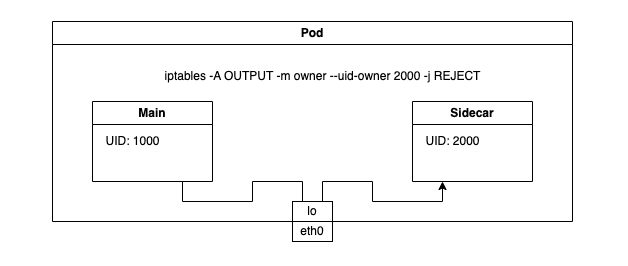
\includegraphics[width=\linewidth]{files/iptables.png}
  \caption{Single network namespace architecture}
  \label{fig:single-net-solution}
\end{figure}

Figure~\ref{fig:single-net-solution} illustrates the network architecture with all required network rule enforcement points. The solution needs to enforce network rules in four scenarios: i) external components and Pod's \texttt{eth0}, ii) main container and \texttt{lo}, iii) sidecar container and \texttt{lo}, and sidecar container and \texttt{eth0}. The ingress and egress rules in the first scenario are more easily enforced with \texttt{NetworkPolicies}, as shown in Listing~\ref{lst:network-policy}. The policies allow cluster and external traffic to the main application port \texttt{8888}, while denying all other traffic into and out of the Pod.

\lstinputlisting[
  caption={Network Policy handling traffic between Pod and external components},
  label={lst:network-policy},
  language={yaml}
]{code/zero-trust-policy.yml}

The other scenarios cannot be enforced with NetworkPolicies, since the rules depend on individual containers instead of Pods. The rules need to be applied inside the Pod's network namespace with tools such as IPTables.

\subsubsection{IPTables}

% TODO: Check process id
Usually, IPTables rules are applied to packets by their IP addresses and ports. However, modern versions of IPTables ship with an owner module, which supports rules based on application's user, group, and session identifiers. For example, \texttt{iptables -A OUTPUT -m owner --uid-owner 1000 -j REJECT} would reject all egress packets from containers with the user id. While the session identifier is assigned at runtime by the kernel, containers' user and group ids can be overridden with Pod definition's \texttt{runAsUser} and \texttt{runAsGroup} fields, respectively. Thus, any ingress or egress traffic of a container with unique user identifier can be filtered with IPTables.

Listing~\ref{lst:iptables-bash} shows IPTables rules that can enforce network rules in other scenarios. As ingress rules, the main application port is opened on all network devices, while the sidecar port is only allowed on the loopback device. For egress traffic, the main application is given access to both containers' ports, while the sidecar can only access its own port. All other traffic is rejected by default.

% need to be applied to Pod's network namespace. Each container receives an own chain. The sidecar container's chain REJECTs all egressing traffic from the sidecar, which prevents the container from accessing any container inside or outside of the Pod. The main application's chain only affects egress traffic to loopback device, and allows traffic only to the port used by the sidecar. Any other egress traffic should be handled by the Network Policy.

\lstinputlisting[
  caption={IPTables rules for the Pod},
  label={lst:iptables-bash},
  language={bash}
]{code/iptables.sh}

The approach is similar to how Istio redirects all Pod traffic through the Envoy sidecar and the service mesh. Istio adds IPTables rules that reroute all traffic, except that which originates from user id 1337, to the Envoy proxy \cite{istio-iptables}. The user id itself is reserved for the proxy, and it is used to avoid re-routing the proxy traffic, which would cause an infinite loop.

eBPF programs were also considered as an option for IPTables. Since XDP programs support only ingress rules, they are not a valid option for solving the problem. However, a TC program that could distinguish sidecar container traffic from others could be a possible option. TC programs manipulate packets by modifying \texttt{struct \_\_sk\_buff} in the user space. The complete C structure is listed as Listing~\ref{lst:sk-buff}.

\lstinputlisting[
  caption={\texttt{skbuff} struct in Linux v6.3 \cite{linux-kernel-skbuff}},
  label={lst:sk-buff},
  language={C}
]{code/skbuff.c}

As can be seen in the example, the structure has no identifiers that are unique for each container. A notable attribute in the structure is the \texttt{mark} field, which can be used as an identifier for the packet in the kernel. It does not propagate with the packet, which means that marking can only be used for traffic filtering before the packet leaves the network stack. If combined with \texttt{iptables} rule that uniquely marks the packets egressing from the sidecar, for example by setting the mark as 2 \texttt{iptables -t mangle -A PREROUTING -m owner --uid-owner 1000 -j MARK --set-mark 2}, a TC eBPF program could be used for filtering the traffic. However, using eBPF brings an extra layer of complexity in comparison to simply using IPtables for traffic filtering. Furthermore, eBPF programs do not provide any performance gains for egressing traffic, since the TC hooks execute after the packet has been processed by IPTables.

\subsubsection{Deployment}

The commands for creating the IPTables rules could be applied to the Pod with the initContainer or postStart lifecycle handler. However, the commands require root user permissions with NET\_ADMIN and NET\_RAW capabilities. Using these methods would require changing Pod's security admission level to privileged. Thus, it is more optimal to apply the rules outside the Pod's context; for example, by using a DaemonSet, similarly to how many CNI plugins configure the Pod network.

\subsection{Own network namespace for sidecar}

% graph TB
%     subgraph "cluster"
%         subgraph "app-pod"
%             eth01(eth0)
%         end
%         subgraph "side-pod"
%             eth02(eth0)
%         end
%         subgraph "kube-system"
%             n1(API)
%         end
%     end

%     subgraph "cluster-external"
%     end

%     eth01<--NetworkPolicy-->cluster-external
%     eth01<--NetworkPolicy-->kube-system
%     eth01<--NetworkPolicy-->eth02
%     eth02<--NetworkPolicy-->cluster-external
%     eth02<--NetworkPolicy-->kube-system

% classDef plain fill:#ddd,stroke:#fff,stroke-width:4px,color:#000;
% classDef k8s fill:#326ce5,stroke:#fff,stroke-width:4px,color:#fff;
% classDef cluster fill:#fff,stroke:#bbb,stroke-width:2px,color:#326ce5;
% class n1,n2,n3,n4 k8s;
% class kube-system,app-ns,cluster-external cluster;

\begin{figure}[h!]
  \centering
  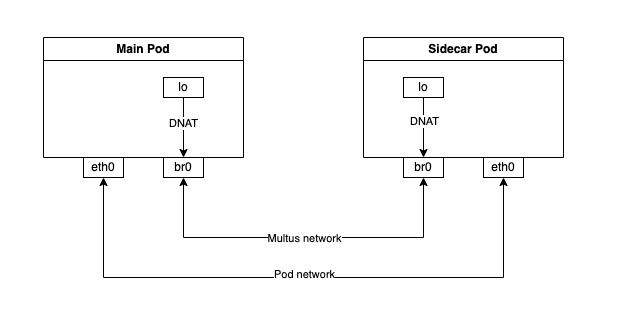
\includegraphics[width=\linewidth]{files/multus.png}
  \caption{Multiple network namespaces architecture}
  \label{fig:multi-pod-net-solution}
\end{figure}

Figure~\ref{fig:multi-pod-net-solution} illustrates the network architecture for the solution in which containers are deployed in different Pods. The idea behind this approach is to use Network Policies for filtering the traffic between the containers. Since containers are not technically sidecars anymore, the solution must recreate communication via the \texttt{localhost} address.

Although it is possible to use the default network created by the CNI plugin for sidecar traffic, the proposed solution creates a new isolated network for traffic with Multus. The isolation allows the use of separate IP address pool, which comes in handy when re-creating the communication via localhost.

\subsubsection{Creating isolated network for sidecar traffic}



It is completely possible to use the default Pod network created by the CNI plugin for traffic between sidecars. With this setup, the network rules are simply Network Policies on top of the policy that implicitly denies all other traffic.

It is also possible to build new network interfaces for sidecar traffic with Multus.

\lstinputlisting[
  caption={NetworkAttachmentDefinition for creating MacVLAN bridge between the Pods},
  label={lst:attachment},
  language={yaml}
]{code/attachment.yml}

The setup requires creating \texttt{NetworkAttachmentDefinition} CRD for the network. Each Pod that should be part of the network needs a \texttt{k8s.v1.cni.cncf.io/networks} annotation, as seen in Listing~\ref{lst:pod-with-bridge}.

\lstinputlisting[
  caption={Deployment with Pod connected to the bridge},
  label={lst:pod-with-bridge},
  language={yaml}
]{code/minimal-deployment.yml}

The common NetworkPolicies are not applied to the Multus network. However, the Multus developers have introduced another CRD, \texttt{MultiNetworkPolicy} \cite{multi-network-policy}, which mimics NetworkPolicies but only works for networks created by Multus. The resource is identical to NetworkPolicies, as seen in the Listing~\ref{lst:policies}.

\lstinputlisting[
  caption={Zero trust MultiNetworkPolicies for br0 network interface},
  label={lst:policies},
  language={yaml}
]{code/multi-network-policies.yml}

However, the Multus CNI does not enforce the \texttt{MultiNetworkPolicy} rules in any way. The implementation is left for other DaemonSets such as \texttt{multi-networkpolicy-iptables} \cite{multi-network-policy-iptables} and \texttt{multi-networkpolicy-tc} \cite{multi-network-policy-tc}, both of which are created by the Multus team. As the names suggest, the DaemonSets implement the enforcement with IPTables and eBPF TC programs, respectively. The \texttt{multi-networkpolicy-iptables} is used for the solution, since \texttt{iptables} implements all other network rules for the cluster.

% TODO: Check security of this https://github.com/kubernetes/kubernetes/issues/90259
% https://security.stackexchange.com/questions/137602/what-are-the-security-implications-of-net-ipv4-conf-eth0-route-localnet-1-rout

With these configurations and dependencies, the containers should have a new network and reach each other via the bridge interface. As the next step, the solution must find a way to redirect the traffic destined for the localhost to the new network. The script in Listing~\ref{lst:dnat} shows how to redirect all egressing traffic with IPTables from the source of \texttt{127.0.0.1:8125} to another network interface with an external IP address, like \texttt{192.168.1.202:8125}. By default, the re-routing of local traffic outside the local machine is denied by the kernel. To overrule this default behavior, the script sets a kernel flag with \lstinline{net.ipv4.conf.all.route_localnet=1}.

\lstinputlisting[
  caption={Script for mapping localhost to br0 interface},
  label={lst:dnat},
  language={bash}
]{code/localhost.sh}

\subsubsection{Mutating sidecars to multiple Pods?}

MutatingAdmissionWebhook?

\clearpage

\section{Solution Evaluation} \label{sec:solution}

\clearpage

\section{Discussion} \label{sec:discussion}

\clearpage

\section{Conclusion} \label{sec:conclusion}

\clearpage

%% Bibliography/ list of references
\thesisbibliography
\printbibliography

%% Appendices
%% If you don't have appendices, your thesis ends here. Remove \clearpage, \thesisappendix and the following text below. The last command of this file is \end{document}.
\clearpage

\thesisappendix

\section{Dockerfile for penetration testing} \label{app:malicious-sidecar}

\lstinputlisting[
  caption={Dockerfile for penetration testing},
  language={Docker}
]{code/appendix/pentest/Dockerfile}

\clearpage

\section{Example webserver deployed with StatsD sidecar} \label{app:node-webapp}

\lstinputlisting[
  caption={Node.js server (\texttt{index.js})},
  language={javascript}
]{code/appendix/app/index.js}

\clearpage

\lstinputlisting[
  caption={\texttt{package.json}},
  language={json}
]{code/appendix/app/package.json}

\lstinputlisting[
  caption={Dockerfile for the server},
  language={Docker}
]{code/appendix/app/Dockerfile}

\clearpage

\section{Webserver and StatsD deployed with Multus networking} \label{app:multus-sidecar}

\lstinputlisting[
  caption={Server's K8s deployment resource},
  language={yaml}
]{code/appendix/multus/node-app.yml}

\clearpage

\lstinputlisting[
  caption={StatsD container's K8s Deployment},
  language={yaml}
]{code/appendix/multus/statsD.yml}

\clearpage

\lstinputlisting[
  caption={Network interfaces and policies},
  language={yaml}
]{code/appendix/multus/interfaces.yml}

\end{document}
